% !TEX encoding = UTF-8 Unicode
%\documentclass[parskip=full,11pt,twoside]{scrartcl}
\documentclass[parskip=full,11pt,twoside]{scrbook}
\usepackage[utf8]{inputenc}

\usepackage[T1]{fontenc}
\usepackage{lmodern}

\usepackage{color}
\usepackage{hyperref}
\usepackage{pdfpages}
\pagestyle{myheadings}

\def\packagename{}
\def\classname{}

% section numbers in margins:
\renewcommand\sectionlinesformat[4]{\makebox[0pt][r]{#3}#4}

% header & footer
\usepackage{scrlayer-scrpage}
\lofoot{\today}
\refoot{\today}
\pagestyle{scrheadings}

\markboth{\protect\packagename{} -- \protect\classname{}}{\protect\packagename{} -- \protect\classname{}}

% hot mess.. I mean.. hotfix
\makeatletter
\DeclareOldFontCommand{\rm}{\normalfont\rmfamily}{\mathrm}
\DeclareOldFontCommand{\sf}{\normalfont\sffamily}{\mathsf}
\DeclareOldFontCommand{\tt}{\normalfont\ttfamily}{\mathtt}
\DeclareOldFontCommand{\bf}{\normalfont\bfseries}{\mathbf}
\DeclareOldFontCommand{\it}{\normalfont\itshape}{\mathit}
\DeclareOldFontCommand{\sl}{\normalfont\slshape}{\@nomath\sl}
\DeclareOldFontCommand{\sc}{\normalfont\scshape}{\@nomath\sc}
\makeatother

\usepackage[sfdefault,light]{roboto}
\usepackage[T1]{fontenc}
\usepackage[german]{babel}
\usepackage[yyyymmdd]{datetime} % must be after babel
\renewcommand{\dateseparator}{-} % ISO8601 date format
\usepackage{hyperref}
\usepackage[nameinlink]{cleveref}
\crefname{figure}{Abb}{Abb}
\usepackage[section]{placeins}
\usepackage{xcolor}
\usepackage{graphicx}
\hypersetup{
	pdftitle={Entwurfsdokumentation},
	bookmarks=true,
}
\usepackage{csquotes}

\usepackage{amsmath} % for $\text{}$
\newcommand\urlpart[2]{$\underbrace{\text{\texttt{#1}}}_{\text{#2}}$}

\renewcommand{\thesection}{\arabic{section}}
% ---------------------------------------------------------------------------
% TexDoc macros start - everything below this point should be copied to your
% own document and adapted to your style/language if needed
% ---------------------------------------------------------------------------

% Environment used to simulate html <p> </p>
\newenvironment{texdocp}{}{

}
% Environment for packages
\newenvironment{texdocpackage}[1]{%
	%\newpage{}
    \gdef\packagename{#1}\subsection{Package \texttt{#1}}
	\rule{\hsize}{.7mm}
}{}


% Environment for classes, interfaces
% Argument 1: "class" or "interface"
% Argument 2: the name of the class/interface
\newenvironment{texdocclass}[2]{%
	\gdef\classname{#2}
	\subsubsection{\texttt{#1 #2}}
}{\newpage{}}

% Environment for class description
\newenvironment{texdocclassintro}{
	\subsubsection*{Description}
}{
}

% Environment around class fields
\newenvironment{texdocclassfields}{%
	\subsubsection*{Attributes}
	\begin{itemize}
}{%
	\end{itemize}
}

% Environment around class methods
\newenvironment{texdocclassmethods}{%
	\subsubsection*{Methods}
	\begin{itemize}
}{%
	\end{itemize}
}

% Environment around class Constructors
\newenvironment{texdocclassconstructors}{%
	\subsubsection*{Constructors}
	\begin{itemize}
}{%
	\end{itemize}
}

% Environment around enum constants
\newenvironment{texdocenums}{%
	\subsubsection*{Enum Constants}
	\begin{itemize}
}{%
	\end{itemize}
}

% Environment around "See also"-Blocks (\texdocsee invocations)
%  Argument 1: Text preceding the references
\newenvironment{texdocsees}[1]{

	\textbf{#1:}
	\begin{itemize}
}{%
	\end{itemize}
}
% Formats a single field
%  Argument 1: modifiers
%  Argument 2: type
%  Argument 3: name
%  Argument 4: Documentation text
\newcommand{\texdocfield}[4]{\item \texttt{#1 #2 \textbf{#3}} \\ #4}

% Formats an enum element
%  Argument 1: name
%  Argument 2: documentation text
\newcommand{\texdocenum}[2]{\item \texttt{\textbf{#1}} \\ #2}

% Formats a single method
%  Argument 1: modifiers
%  Argument 2: return type
%  Argument 3: name
%  Argument 4: part after name (parameters)
%  Argument 5: Documentation text
%  Argument 6: Documentation of parameters/exceptions/return values
\newcommand{\texdocmethod}[6]{\item \texttt{#1 #2 \textbf{#3}#4} \\ #5#6}

% Formats a single constructor
%  Argument 1: modifiers
%  Argument 2: name
%  Argument 3: part after name (parameters)
%  Argument 4: Documentation text
%  Argument 5: Documentation of parameters/exceptions/return values
\newcommand{\texdocconstructor}[5]{\item \texttt{#1 \textbf{#2}#3} \\ #4#5}

% Inserted when @inheritdoc is used
%  Argument 1: Class where the documentation was inherited from
%  Argument 2: Documentation
\newcommand{\texdocinheritdoc}[2]{#2 (\textit{documentation inherited from \texttt{#1})}}

% Formats a single see-BlockTag
%  Argument 1: text
%  Argument 2: reference label
\newcommand{\texdocsee}[2]{\item \texttt{#1 (\ref{#2})}}

% Environment around \texdocparameter invocations
\newenvironment{texdocparameters}{%
	\minisec{Parameters}
	\begin{tabular}{ll}
}{%
	\end{tabular}
}

% Environment around \texdocthrow invocations
\newenvironment{texdocthrows}{%
        \minisec{Throws}
        \begin{tabular}{ll}
}{%
        \end{tabular}
}

\newcommand{\texdocreturn}[1]{\minisec{Returns} #1}

% Formats a parameter (this gets put inside the input of a \texdocmethod or
% \texdocconstructor macro)
%  Argument 1: name
%  Argument 2: description text
\newcommand{\texdocparameter}[2]{\texttt{\textbf{#1}} & \begin{minipage}[t]{0.8\textwidth}#2\end{minipage} \\}

% Formats a throws tag
%  Argument 1: exception name
%  Argument 2: description text
\newcommand{\texdocthrow}[2]{\texttt{\textbf{#1}} & \begin{minipage}[t]{0.6\textwidth}#2\end{minipage} \\}

% Used to simulate html <br/>
\newcommand{\texdocbr}{\mbox{}\newline{}}

% Used to simulate html <h[1-9]> - </h[1-9]>
% Argument 1: number of heading (5 for a <h5>)
% Argument 2: heading text
\newcommand{\headref}[2]{\minisec{#2}}

\newcommand{\refdefined}[1]{
\expandafter\ifx\csname r@#1\endcsname\relax
\relax\else
{$($ in \ref{#1}, page \pageref{#1}$)$}
\fi}

% ---------------------------------------------------------------------------
% TexDoc macros end
% ---------------------------------------------------------------------------




\begin{titlepage}

\subject{Entwurfsdokumentation}
\title{$\lambda$urora}
\subtitle{The Lambda Calculus IDE}


\author{Iuliia Patrusheva, Alexander von Heyden\\
Younis Bensalah, Max Nowak\\
Nikolai Polley, Randy Seng}

\end{titlepage}




\begin{document}
\maketitle
\pagebreak
%dontbreak
\setcounter{tocdepth}{4}
\tableofcontents

\newpage
\section{Einleitung}

\subsection{Zweck der Software}
Ziel der Software Aurora ist es, Studenten eine Lernumgebung zu bieten, in der sie mit eigenen Lambda Termen sowohl arbeiten als auch experimentieren können.
Hierdurch soll es den Studenten ermöglicht werden, ein besseres Gefühl für das $\lambda$-Kalkül zu entwickeln.
Hilfestellungen werden neben farbiger Hervorhebung der Termstrukturen auch durch eine anschauliche Darstellung von Zwischenschritte gegeben.
Darüberhinaus existiert eine vordefinierte Standardbibliothek, in der häufig benutzte Funktionen und Church Zahlen (in numerischer Schreibweise) vordefiniert sind.
\newline
Weitere Features sind unter anderem das einfache Erstellen von Lernmaterial durch einen \LaTeX-Export, als auch das Teilen des eigenen Inputs, inklusive dazugehöriger Benutzerbibliothek.

\subsection{Entwurfsziele}
Die Erstellung dieses Entwurfes hatte folgende Zielsetzungen:
\begin{description}
	
		\item[\textbf{Geheimhaltungsprinzip}] ~\par
			Klassen geben so wenig Informationen wie möglich über Implementierungsdetails preis.
			
		\item[\textbf{Starke Kohäsion in Pakete und Klassen}] ~\par
			Eine Klasse hat nur Methoden, die sie direkt betrifft. 
            Klassen innerhalb eines Paketes werden meist zusammen benutzt.
			
		\item[\textbf{Lose Koppelung zwischen Klassen und Paketen}]~\par
			Eine Klassen kennt so wenig wie mögliche andere Klassen.
			
		\item[\textbf{Lokalitätsprinzip beachten}] ~\par
			Eine Klasse soll auch alleine stehend verständlich sein.
            Die Klasse Term ist eine Ausnahme, da sie im Backend nahezu allen bekannt sein muss (siehe Abgrenzungskriterium \textbf{A3}).
            Deswegen ist die Klasse Term abstrakt, und sehr schlank gehalten.
			
		\item[\textbf{Keine Verwendung von instanceof}] ~\par
            Auch als sich \enquote{instanceof} als Entwurfsentscheidung sehr gut angeboten hat, haben wir eine andere Methode gewählt.
	
\end{description}
\pagebreak

\section{Grobentwurf}
\subsection{Architekturmuster und Systemzerlegung}
\subsubsection{Übersicht}
Bei dem Programm handelt es sich um eine clientseitige Anwendung, die auf \enquote{Google Chrome} 62 lauffähig ist.
Unter der Voraussetzung, dass in PSE eine objektorientierte Sprache verwendet werden muss, haben wir uns für Java 8 entschieden.
Damit unser Programm in Chrome ausgeführt werden kann, haben wir uns für die Verwendung des \enquote{Google Web Toolkits} entschieden (\enquote{GWT});
Dieses erlaubt es uns, Java Sourcecode nach Javascript zu übersetzen.
\newline
Aurora ist ein klassische aufgebautes Programm.
Somit besteht es aus einer GUI, in die der Benutzer seinen Input eingeben kann, und einem Backend, in dem alle benötigten Berechnungen durchgeführt werden. 
In der Vorlesung \enquote{Softwaretechnik I} wurde für dieses Szenario das Muster \enquote{Model-View-Controller} vorgestellt.
Im Gegensatz dazu haben wir uns allerdings für \enquote{Model-View-Presenter} entschieden, was vorallem daran liegt, dass \enquote{GWT} mit \enquote{MVP} im Kopf entworfen wurde.
Es wäre  zwar auch möglich gewesen \enquote{MVC} zu wählen, allerdings würden sich hier vor allem beim Schreiben von Testcases Schwierigkeiten auftun.
Die Verwendung von \enquote{MVP} erlaubt in großen Teilen das Ausführen von klassischen Java Tests;
Bei \enquote{MVC} wäre dies nicht so einfach möglich, hier müsste man die Tests speziell an \enquote{GWT} anpassen, was unter anderem zu einer längeren Laufzeit der Teste führen würde.

\subsubsection{Model-View-Presenter}
\enquote{MVP} ist ein Entwurfsmuster, welches aus drei Komponenten besteht, Model, View, und Presenter.
\begin{description}
	\item[Model] ~\par
	Das Model beinhaltet die Logik und alle Funktionalität der View.
    Im Gegensatz zum \enquote{MVC} hat hier das Model weder Zugriff auf die View, noch auf den Presenter.

	\item[View] ~\par
	Die View wird für das Darstellen der Ein- und Ausgaben benutzt.
    Somit ist die grafische Oberfläche des Programms ein Teil der View;
    Sie enthält aber keinerlei Logik und kennt weder das Model noch den Presenter.
	
	\item[Presenter] ~\par
	Der Presenter kennt sowohl View als auch das Model und verknüpft ihre Funktionen.
    Er steuert die Kommunikation zwischen den zwei Komponenten und koordiniert die logischen Abläufe.
\end{description}

\subsubsection{Lambda-Bibliothek}
Ein Teil des Projektes kann als eigene Lambda-Bibliothek betrachtet werden.
Im Code wird diese Eigenschaft nicht explizit sichtbar gemacht, lediglich ein eigenes Package weist darauf hin;
Bei Bedarf könnte es jedoch in eine externe Bibliothek ausgelagert, und anschließend in Aurora eingebunden werden.
Diese \enquote{Bibliothek} existiert, um den Umgang mit Lambda-Termen zu erleichtern.
Sie implementiert unter anderem Funktionalität zum Beta-Reduzieren, Substituieren von Variablen, Finden von Redexen, sowie verschiedene Auswertungsstrategien von Lambda-Termen.

\subsection{Paketbeschreibungen}
\begin{description}
	
	
	\item[aurora] ~\par
	Alle Pakete und Klassen sind in diesem Oberpaket definiert.
	
	\item[aurora.backend] ~\par
	Im Backend sind alle Berechnungen und Datenstrukturen, die für das Lambda Kalkül gebraucht werden. 
	
	\item[aurora.backend.parser] ~\par
	In diesem Paket wird eine Eingabe geparsed.
	
	\item[aurora.backend.parser.exceptions] ~\par
	Die Exceptions, die bei beim Parsen geworfen werden können.
	
	\item[aurora.backend.tree] ~\par
	Dies ist die grundlegende Datenstruktur, in der die Lambdaterme gespeichert werden.
	
	\item[aurora.backend.library] ~\par
	Dieses Paket wird für die Benutzer- und Standardbibliothek benutzt.
	
	\item[aurora.backend.librarby.exceptions] ~\par
	Die Exceptions, die bei der Library geworfen werden können.
	
	\item[aurora.backend.betareduction] ~\par
	Dieses Paket umfasst alles, was für die Beta-Reduktion benötigt wird.
	
	\item[aurora.backend.betareduction.visitors] ~\par
	In diesem Paket sind die Besucher, welche den Tree traversieren.
	Sie werden für die Beta-Reduktion benötigt.
	
	\item[aurora.backend.betareduction.strategies] ~\par
	Hier liegen alle Reduktionsstrategien die für die Beta-Reduktion benutzt werden können.
	
	\item[aurora.backend.encoders] ~\par
	Das Paket wird für das Encoden und Decoden des Inputs benutzt.
	
	\item[aurora.backend.encoders.exceptions] ~\par
	Die Exceptions, die beim Encoden/Decoden geworfen werden können.
	
	\item[aurora.backend.simplifier] ~\par
	In diesem Paket wird versucht, einen komplexer Term in eine simple Ausgabe zu überführen.
	
	\item[aurora.client] ~\par
	Hier sind alle Funktionen, die für den Client benötigt werden.
	
	\item[aurora.client.event] ~\par
	Das Paket beinhaltet alle Events, die ausgelöst werden können.
	
	\item[aurora.client.view] ~\par
	Hier liegt die GUI.
	
	\item[aurora.client.view.editor] ~\par
	Der Editor für die Benutzereingabe.
	
	\item[aurora.client.view.editor.actionbar] ~\par
	Die Actionbar des Editors.
	
	\item[aurora.client.view.popup] ~\par
	Dieses Paket beinhaltet alle Popups.
	
	\item[aurora.client.view.sidebar] ~\par
	An der linken Seite der GUI ist eine Sidebar.
	Sie wird von diesem Paket bereitgestellt.
	
	\item[aurora.client.view.sidebar.strategy] ~\par 
	Die Strategieauswahl in der Sidebar.
	
	\item[aurora.client.presenter] ~\par
	Der Presenter, der den Daten- und Kontrollfluss steuert.
	
\end{description}


\subsection{Entwurfsmuster}
Für das Traversieren der Terme wird das Visitor Pattern (Besucher) benutzt. Es werden jeweils konkrete Besucher erstellt, die jeweils unterschiedliche Funktionen besitzen um den Term auszuwerten.

Die Sidebar verwendet das Entwurfsmuster Kompositum.

Das Eventhandling wird mit Observern vollzogen.

%\pagebreak

\newpage
\section{Sequenzdiagramme}
\subsection{AppLaunch}
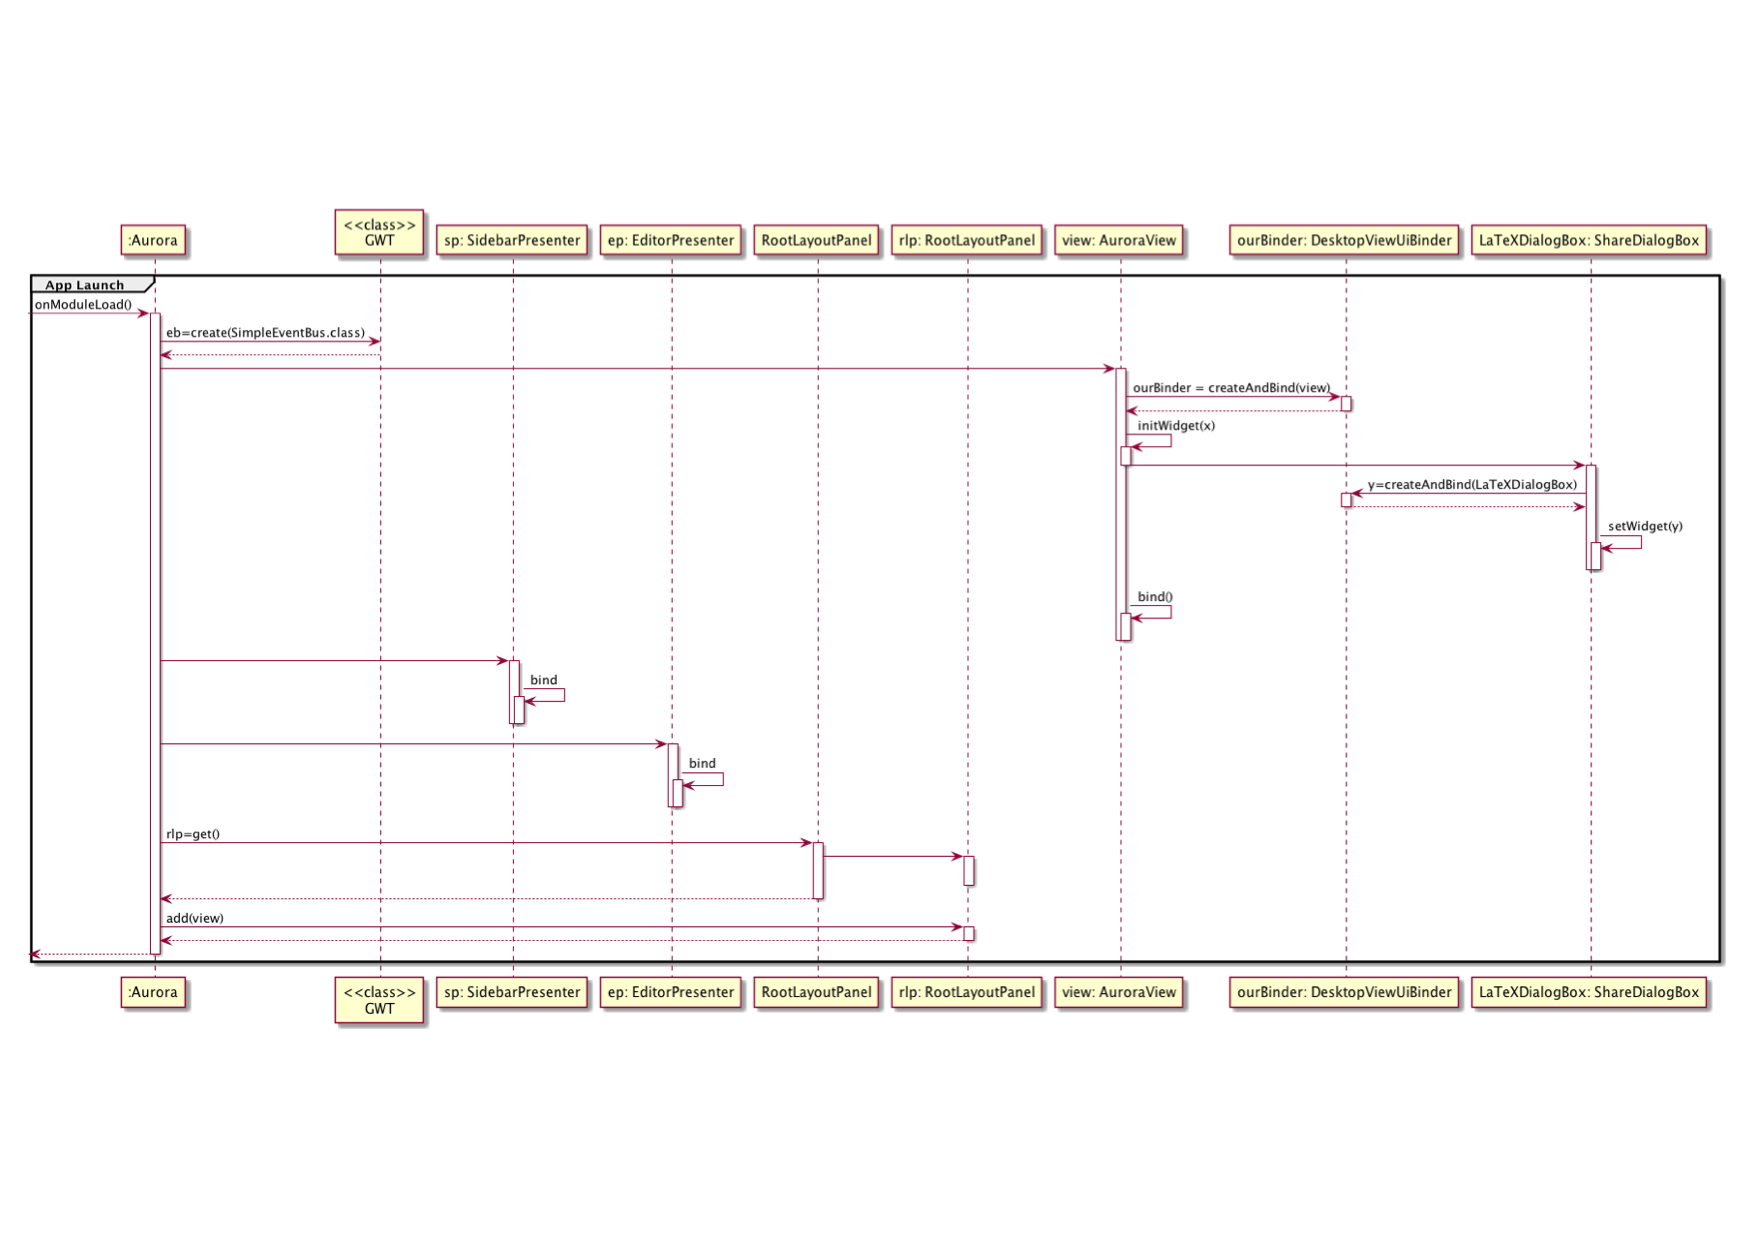
\includegraphics[width=0.75\textwidth]{../uml/SD/AppLaunch.png}
\subsection{Share LaTeX}
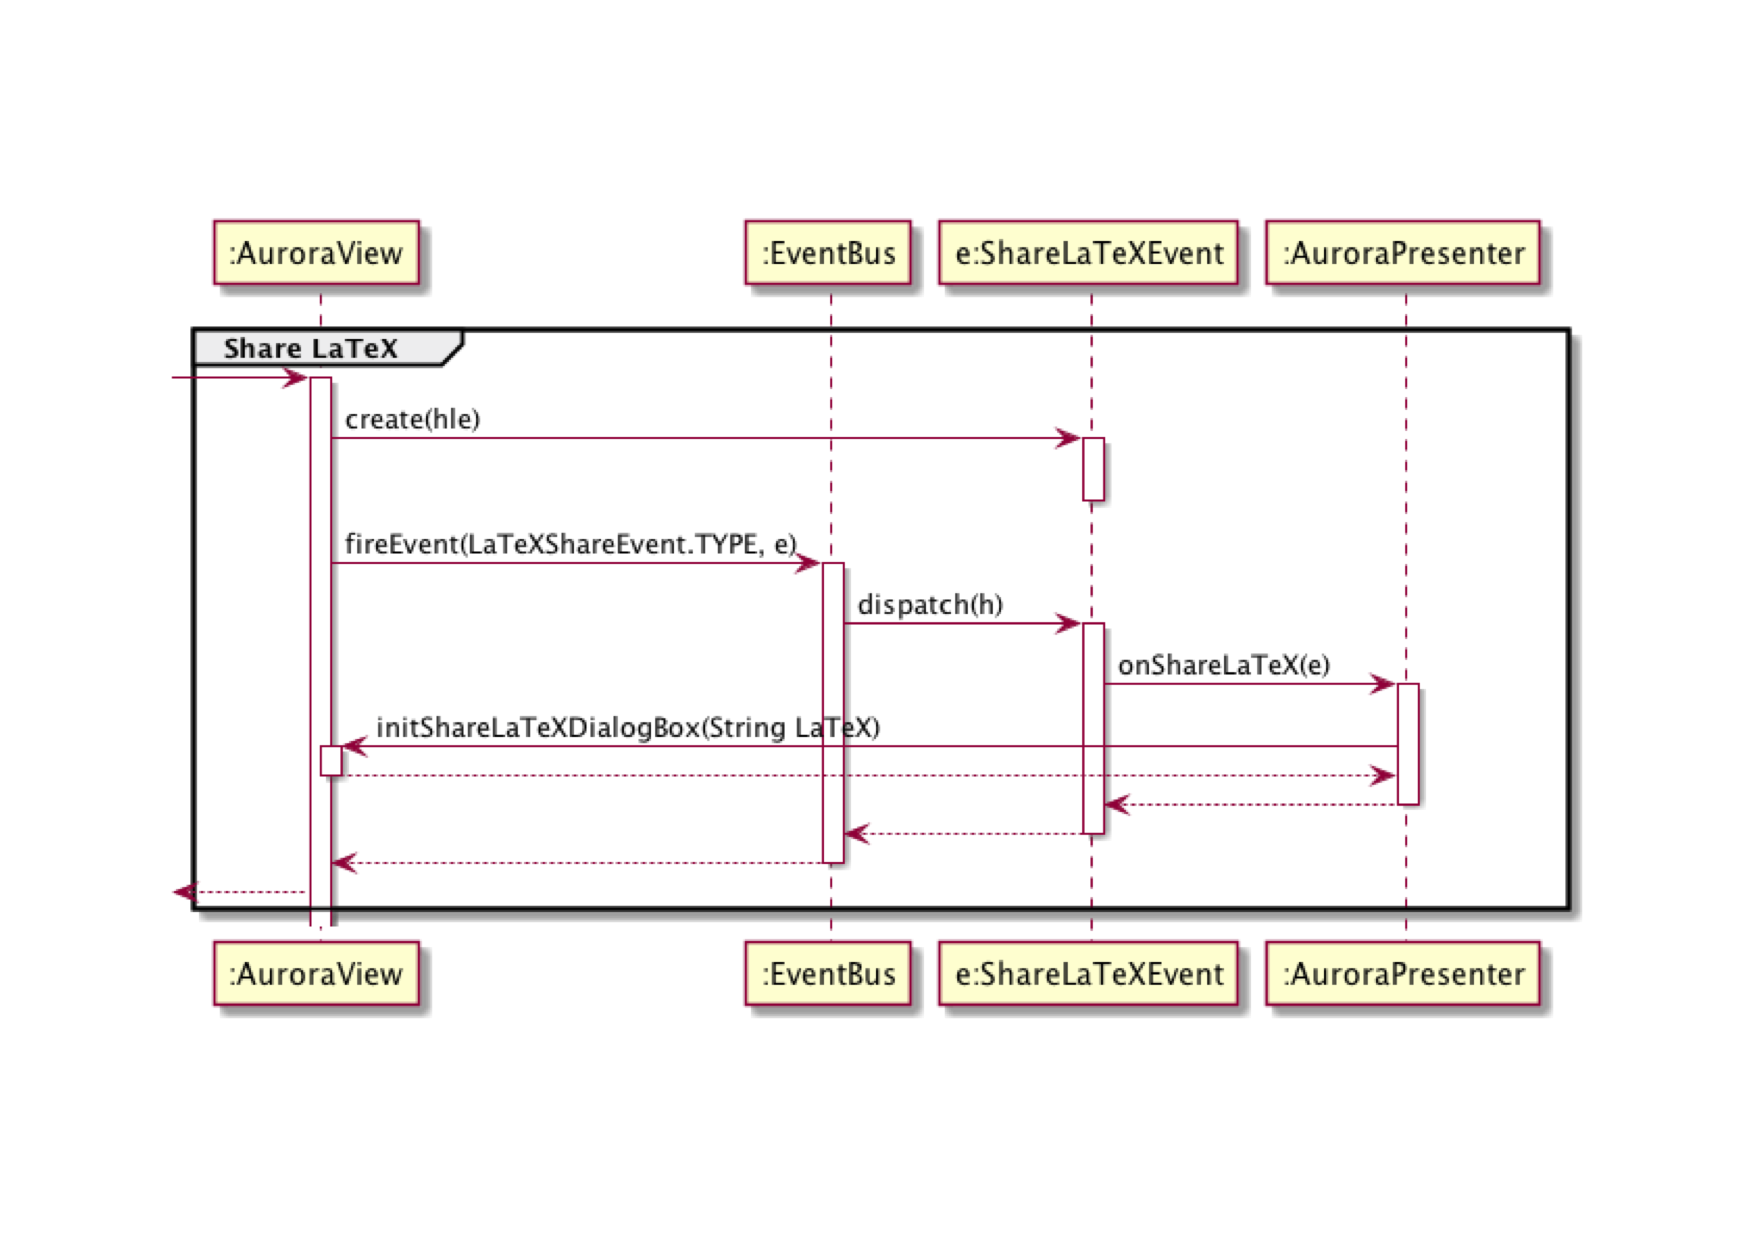
\includegraphics[width=0.75\textwidth]{../uml/SD/ShareLaTeX.png}
\subsection{Step interaction}
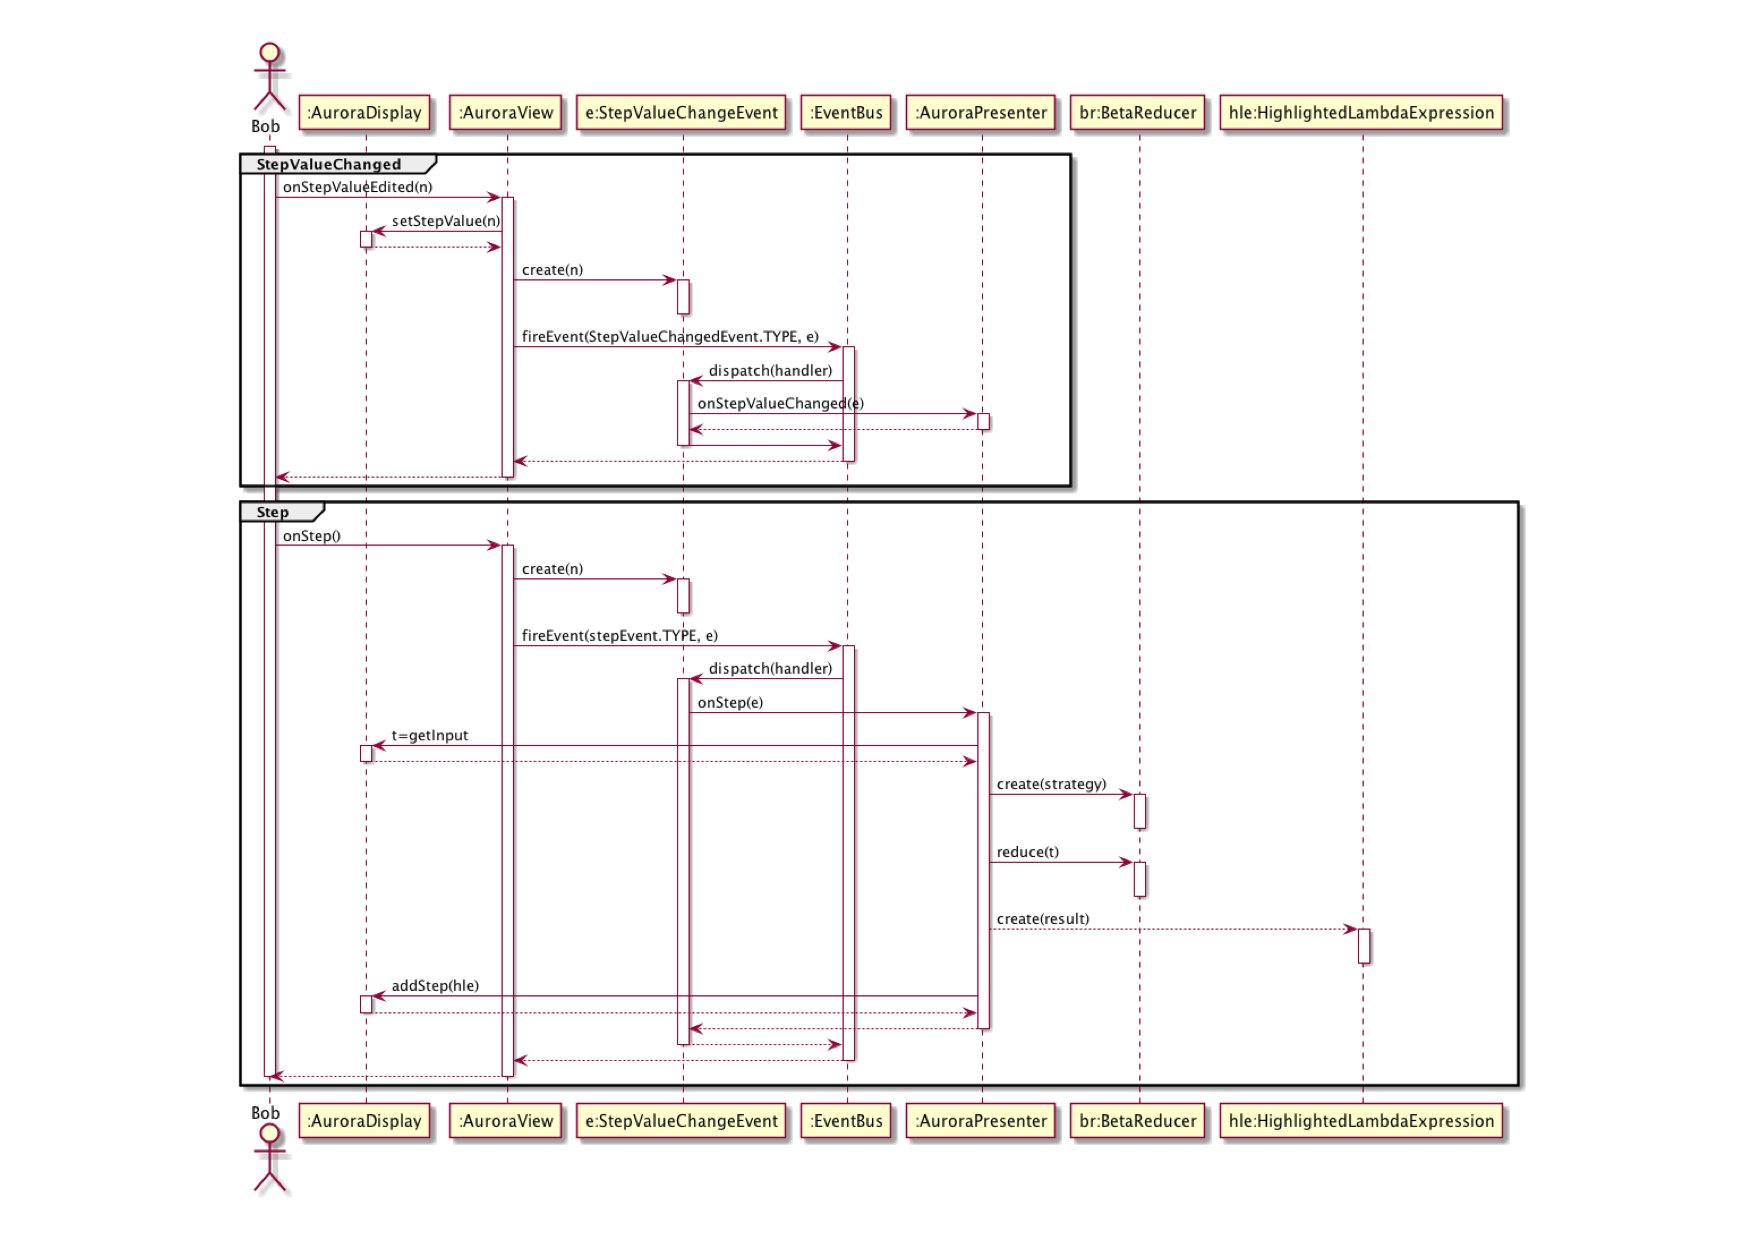
\includegraphics[width=0.75\textwidth]{../uml/SD/StepInteraction.png}

\newpage
\section{Feinentwurf}


%\newpage
\subsection{Klassen und Schnittstellen}
% include crap from texdoclet
%\tableofcontents
\begin{texdocpackage}{aurora.backend}
\label{texdoclet:aurora.backend}

\begin{texdocclass}{class}{HighlightableLambdaExpression}{}{HighlightedLambdaExpression}
\label{texdoclet:aurora.backend.HighlightableLambdaExpression}
\begin{texdocclassintro}
Encapsulates the lambda term combined with meta information about highlighting.\end{texdocclassintro}
\begin{texdocclassconstructors}
\texdocconstructor{public}{HighlightableLambdaExpression}{()}{Standard constructor that initializes with an empty Token (see \ref{texdoclet:aurora.backend.parser.Token}) list.}{}
\texdocconstructor{public}{HighlightableLambdaExpression}{(List\textless{}Token\textgreater{} stream)}{Constructor that creates a HighlightableLambdaExpression (see \ref{texdoclet:aurora.backend.HighlightableLambdaExpression}) from a stream of Token (see \ref{texdoclet:aurora.backend.parser.Token})s.}{\begin{texdocparameters}
\texdocparameter{stream}{The Token (see \ref{texdoclet:aurora.backend.parser.Token}) stream.}
\end{texdocparameters}
}
\texdocconstructor{public}{HighlightableLambdaExpression}{(Term t)}{Constructor that analyzes a Term (see \ref{texdoclet:aurora.backend.tree.Term}) and creates the HighlightableLambdaExpression (see \ref{texdoclet:aurora.backend.HighlightableLambdaExpression}).}{\begin{texdocparameters}
\texdocparameter{t}{The Term (see \ref{texdoclet:aurora.backend.tree.Term}) that gets analyzed.}
\end{texdocparameters}
}
\end{texdocclassconstructors}
\begin{texdocclassmethods}
\texdocmethod{public}{List\textless{}HighlightedLambdaExpression.Redex\textgreater{}}{getAllRedexes}{()}{}{}
\texdocmethod{public}{HighlightedLambdaExpression.Redex}{getNextRedex}{()}{}{}
\texdocmethod{public}{HighlightedLambdaExpression.Redex}{getPreviousRedex}{()}{}{}
\texdocmethod{public}{RedexPath}{getRedexPathFromToken}{(Token token)}{}{\begin{texdocparameters}
\texdocparameter{token}{}
\end{texdocparameters}
\texdocreturn{}
}
\texdocmethod{public}{void}{highlightNextRedex}{(HighlightedLambdaExpression.Redex redex)}{}{}
\texdocmethod{public}{void}{highlightPreviousRedex}{(HighlightedLambdaExpression.Redex redex)}{}{}
\texdocmethod{public}{void}{highlightRedex}{(HighlightedLambdaExpression.Redex redex)}{}{}
\texdocmethod{public}{Iterator\textless{}Token\textgreater{}}{iterator}{()}{}{}
\texdocmethod{public}{String}{toString}{()}{}{}
\end{texdocclassmethods}
\end{texdocclass}


\begin{texdocclass}{interface}{HighlightedLambdaExpression}{}{Iterable}
\label{texdoclet:aurora.backend.HighlightedLambdaExpression}
\begin{texdocclassintro}
A read-only version of HighlightableLambdaExpression.\end{texdocclassintro}
\begin{texdocclassmethods}
\texdocmethod{public}{List\textless{}HighlightedLambdaExpression.Redex\textgreater{}}{getAllRedexes}{()}{Get all possible redexes.}{\texdocreturn{}
}
\texdocmethod{public}{HighlightedLambdaExpression.Redex}{getNextRedex}{()}{Gets the redex that will be executed in the next step.}{\texdocreturn{}
}
\texdocmethod{public}{HighlightedLambdaExpression.Redex}{getPreviousRedex}{()}{Gets the redex resulting from the previous computation. Or null.}{\texdocreturn{Redex.}
}
\texdocmethod{public}{Iterator\textless{}Token\textgreater{}}{iterator}{()}{}{}
\end{texdocclassmethods}
\end{texdocclass}


\begin{texdocclass}{class}{HighlightedLambdaExpression.Redex}{}{}
\label{texdoclet:aurora.backend.HighlightedLambdaExpression.Redex}
\begin{texdocclassintro}
Represents a redex in a specific tree. Information contained depends on that specific tree, and consists of
 Token indices and a RedexPath.\end{texdocclassintro}
\begin{texdocclassfields}
\texdocfield{public final}{int}{lastToken}{The last token of the right side of the application.}
\texdocfield{public final}{int}{middleToken}{The first token of the right side of the application.}
\texdocfield{public final}{RedexPath}{redex}{Associated path to this redex in the specific tree this Redex belongs to.}
\texdocfield{public final}{int}{startToken}{The very first token of the Redex. Usually a lambda.}
\end{texdocclassfields}
\begin{texdocclassconstructors}
\texdocconstructor{public}{Redex}{(int startToken, int middleToken, int lastToken, RedexPath redex)}{Creates a new Redex.}{\begin{texdocparameters}
\texdocparameter{startToken}{Start.}
\texdocparameter{middleToken}{Middle.}
\texdocparameter{lastToken}{End.}
\texdocparameter{redex}{Redex path.}
\end{texdocparameters}
}
\end{texdocclassconstructors}
\end{texdocclass}


\begin{texdocclass}{class}{MetaTerm}{aurora.backend.tree.Term}{}
\label{texdoclet:aurora.backend.MetaTerm}
\begin{texdocclassintro}
Special kind of Term (see \ref{texdoclet:aurora.backend.tree.Term}) that keeps track of meta information about where it came from.
 A MetaTerm (see \ref{texdoclet:aurora.backend.MetaTerm}) is a wrapper around a Term (see \ref{texdoclet:aurora.backend.tree.Term}) that carries a reference to a concrete Token (see \ref{texdoclet:aurora.backend.parser.Token}) object.\end{texdocclassintro}
\begin{texdocclassfields}
\texdocfield{public final}{Term}{term}{Inner Term (see \ref{texdoclet:aurora.backend.tree.Term}).}
\texdocfield{public final}{Token}{token}{Associated Token (see \ref{texdoclet:aurora.backend.parser.Token}).}
\end{texdocclassfields}
\begin{texdocclassconstructors}
\texdocconstructor{public}{MetaTerm}{(Term term, Token token)}{Constructor that initializes a MetaTerm (see \ref{texdoclet:aurora.backend.MetaTerm}) with an inner Term (see \ref{texdoclet:aurora.backend.tree.Term}) and an associated Token (see \ref{texdoclet:aurora.backend.parser.Token}).}{\begin{texdocparameters}
\texdocparameter{term}{The inner Term (see \ref{texdoclet:aurora.backend.tree.Term}).}
\texdocparameter{token}{The associated Token (see \ref{texdoclet:aurora.backend.parser.Token}).}
\end{texdocparameters}
}
\end{texdocclassconstructors}
\begin{texdocclassmethods}
\texdocmethod{public}{T}{accept}{(TermVisitor\textless{}T\textgreater{} visitor)}{}{}
\end{texdocclassmethods}
\end{texdocclass}


\begin{texdocclass}{class}{RedexPath}{}{Iterable}
\label{texdoclet:aurora.backend.RedexPath}
\begin{texdocclassintro}
A RedexPath (see \ref{texdoclet:aurora.backend.RedexPath}) is a series of left and right instructions that point to an Application (see \ref{texdoclet:aurora.backend.tree.Application}) within a tree of Term (see \ref{texdoclet:aurora.backend.tree.Term})s.\end{texdocclassintro}
\begin{texdocclassconstructors}
\texdocconstructor{public}{RedexPath}{()}{This constructor initializes an empty RedexPath (see \ref{texdoclet:aurora.backend.RedexPath}).}{}
\end{texdocclassconstructors}
\begin{texdocclassmethods}
\texdocmethod{public}{Application}{get}{(Term term)}{A Term (see \ref{texdoclet:aurora.backend.tree.Term}) gets traversed like the RedexPath (see \ref{texdoclet:aurora.backend.RedexPath}) describes and returns the Application (see \ref{texdoclet:aurora.backend.tree.Application}) that it points to.}{\begin{texdocparameters}
\texdocparameter{term}{The term that will get traversed.}
\end{texdocparameters}
\texdocreturn{The Application (see \ref{texdoclet:aurora.backend.tree.Application}) that we're pointing to.}
}
\texdocmethod{public}{Iterator\textless{}RedexPath.Direction\textgreater{}}{iterator}{()}{}{}
\texdocmethod{public}{void}{pop}{()}{Deletes the last element of the list.}{}
\texdocmethod{public}{void}{push}{(RedexPath.Direction d)}{Add a new enum to the List.}{\begin{texdocparameters}
\texdocparameter{d}{The enum left or right.}
\end{texdocparameters}
}
\end{texdocclassmethods}
\end{texdocclass}


\begin{texdocclass}{enum}{RedexPath.Direction}{}{}
\label{texdoclet:aurora.backend.RedexPath.Direction}
\begin{texdocclassintro}
Indicate the direction during tree traversal.\end{texdocclassintro}
\begin{texdocenums}
\texdocenum{LEFT}{}
\texdocenum{RIGHT}{}
\end{texdocenums}
\begin{texdocclassmethods}
\texdocmethod{public static}{RedexPath.Direction}{valueOf}{(String name)}{}{}
\texdocmethod{public static}{RedexPath.Direction}{values}{()}{}{}
\end{texdocclassmethods}
\end{texdocclass}


\begin{texdocclass}{class}{ShareLaTeX}{}{}
\label{texdoclet:aurora.backend.ShareLaTeX}
\begin{texdocclassintro}
This class generates a LaTeX snippet which can be pasted into a LaTeX document.\end{texdocclassintro}
\begin{texdocclassconstructors}
\texdocconstructor{public}{ShareLaTeX}{(HighlightedLambdaExpression hle)}{Traverse the HighlightableLambdaExpression.}{\begin{texdocparameters}
\texdocparameter{hle}{The highlighted lambda expression.}
\end{texdocparameters}
}
\end{texdocclassconstructors}
\begin{texdocclassmethods}
\texdocmethod{public}{String}{generateLaTeX}{()}{Creates a LaTeX snippet as a string which can be copied into a LaTeX document.}{\texdocreturn{A string which contains the LaTeX code.}
}
\end{texdocclassmethods}
\end{texdocclass}


\begin{texdocclass}{class}{TermVisitor}{}{}
\label{texdoclet:aurora.backend.TermVisitor}
\begin{texdocclassintro}
Term tree Visitor with generic return type.\end{texdocclassintro}
\begin{texdocclassconstructors}
\texdocconstructor{public}{TermVisitor}{()}{}{}
\end{texdocclassconstructors}
\begin{texdocclassmethods}
\texdocmethod{public abstract}{T}{visit}{(Abstraction abs)}{Called with Abstraction (see \ref{texdoclet:aurora.backend.tree.Abstraction}).}{\begin{texdocparameters}
\texdocparameter{abs}{The caller.}
\end{texdocparameters}
\texdocreturn{Result or null.}
}
\texdocmethod{public abstract}{T}{visit}{(Application app)}{Called with Application (see \ref{texdoclet:aurora.backend.tree.Application}).}{\begin{texdocparameters}
\texdocparameter{app}{The caller.}
\end{texdocparameters}
\texdocreturn{Result or null.}
}
\texdocmethod{public abstract}{T}{visit}{(BoundVariable bvar)}{Called by BoundVariable (see \ref{texdoclet:aurora.backend.tree.BoundVariable}).}{\begin{texdocparameters}
\texdocparameter{bvar}{The caller.}
\end{texdocparameters}
\texdocreturn{Result or null.}
}
\texdocmethod{public abstract}{T}{visit}{(FreeVariable fvar)}{Called with FreeVariable (see \ref{texdoclet:aurora.backend.tree.FreeVariable}).}{\begin{texdocparameters}
\texdocparameter{fvar}{The caller.}
\end{texdocparameters}
\texdocreturn{Result or null.}
}
\texdocmethod{public abstract}{T}{visit}{(LibraryTerm libterm)}{Called with LibraryTerm (see \ref{texdoclet:aurora.backend.tree.LibraryTerm}).}{\begin{texdocparameters}
\texdocparameter{libterm}{The caller.}
\end{texdocparameters}
\texdocreturn{Result or null.}
}
\texdocmethod{public abstract}{T}{visit}{(ChurchNumber c)}{Called with ChurchNumber (see \ref{texdoclet:aurora.backend.tree.ChurchNumber}).}{\begin{texdocparameters}
\texdocparameter{c}{The caller.}
\end{texdocparameters}
\texdocreturn{Result or null.}
}
\texdocmethod{public}{T}{visit}{(MetaTerm mt)}{Called with MetaTerm (see \ref{texdoclet:aurora.backend.MetaTerm}).
 The default implementation is to just skip any MetaTerm (see \ref{texdoclet:aurora.backend.MetaTerm}).}{\begin{texdocparameters}
\texdocparameter{mt}{}
\end{texdocparameters}
\texdocreturn{}
}
\end{texdocclassmethods}
\end{texdocclass}


\end{texdocpackage}



\begin{texdocpackage}{aurora.backend.betareduction}
\label{texdoclet:aurora.backend.betareduction}

\begin{texdocclass}{class}{BetaReducer}{}{}
\label{texdoclet:aurora.backend.betareduction.BetaReducer}
\begin{texdocclassintro}
\end{texdocclassintro}
\begin{texdocclassconstructors}
\texdocconstructor{public}{BetaReducer}{(ReductionStrategy strategy)}{The constructor gets a strategy that is used for the reduction.}{\begin{texdocparameters}
\texdocparameter{strategy}{The chosen reduction strategy.}
\end{texdocparameters}
}
\end{texdocclassconstructors}
\begin{texdocclassmethods}
\texdocmethod{public}{Term}{reduce}{(Term term)}{This method performs one beta reduction.}{\begin{texdocparameters}
\texdocparameter{term}{The Term that will get reduced.}
\end{texdocparameters}
\texdocreturn{null if not reducible, otherwise reduced Term.}
}
\end{texdocclassmethods}
\end{texdocclass}


\end{texdocpackage}



\begin{texdocpackage}{aurora.backend.betareduction.strategies}
\label{texdoclet:aurora.backend.betareduction.strategies}

\begin{texdocclass}{class}{CallByName}{ReductionStrategy}{}
\label{texdoclet:aurora.backend.betareduction.strategies.CallByName}
\begin{texdocclassintro}
This is the Call By Name Strategy. The Strategy reduces the leftmost redex, when not enclosed by an abstraction.
 This will be made by a depth first search, that doesn't go below abstractions.\end{texdocclassintro}
\begin{texdocclassconstructors}
\texdocconstructor{public}{CallByName}{()}{}{}
\end{texdocclassconstructors}
\begin{texdocclassmethods}
\texdocmethod{public}{RedexPath}{getRedex}{(Term t)}{}{}
\end{texdocclassmethods}
\end{texdocclass}


\begin{texdocclass}{class}{CallByValue}{ReductionStrategy}{}
\label{texdoclet:aurora.backend.betareduction.strategies.CallByValue}
\begin{texdocclassintro}
This is the Call By Value strategy. It reduces an abstraction which has a "value" as it's parameter. A value is an abstraction or a free variable.\end{texdocclassintro}
\begin{texdocclassconstructors}
\texdocconstructor{public}{CallByValue}{()}{}{}
\end{texdocclassconstructors}
\begin{texdocclassmethods}
\texdocmethod{public}{RedexPath}{getRedex}{(Term t)}{}{}
\end{texdocclassmethods}
\end{texdocclass}


\begin{texdocclass}{class}{NormalOrder}{ReductionStrategy}{}
\label{texdoclet:aurora.backend.betareduction.strategies.NormalOrder}
\begin{texdocclassintro}
The Normalorder is the default reduction strategy, it choses the leftmost redex.\end{texdocclassintro}
\begin{texdocclassconstructors}
\texdocconstructor{public}{NormalOrder}{()}{}{}
\end{texdocclassconstructors}
\begin{texdocclassmethods}
\texdocmethod{public}{RedexPath}{getRedex}{(Term t)}{}{}
\end{texdocclassmethods}
\end{texdocclass}


\begin{texdocclass}{class}{ReductionStrategy}{}{}
\label{texdoclet:aurora.backend.betareduction.strategies.ReductionStrategy}
\begin{texdocclassintro}
A beta reduction strategy.\texdocbr  A strategy evaluates terms and choses a redex to be reduced by the BetaReducer (see \ref{texdoclet:aurora.backend.betareduction.BetaReducer}).
 The location within the Term tree is given via a RedexPath (see \ref{texdoclet:aurora.backend.RedexPath}) object.\end{texdocclassintro}
\begin{texdocclassconstructors}
\texdocconstructor{public}{ReductionStrategy}{()}{}{}
\end{texdocclassconstructors}
\begin{texdocclassmethods}
\texdocmethod{public abstract}{RedexPath}{getRedex}{(Term t)}{A strategy evaluates terms and choses a redex which gets reduced by the BetaReducer (see \ref{texdoclet:aurora.backend.betareduction.BetaReducer}).
 The Strategies return a treepath which show the chosen redex.}{\begin{texdocparameters}
\texdocparameter{t}{the term which gets evaluated.}
\end{texdocparameters}
\texdocreturn{the tree path to the chosen redex.}
}
\end{texdocclassmethods}
\end{texdocclass}


\begin{texdocclass}{class}{UserStrategy}{ReductionStrategy}{}
\label{texdoclet:aurora.backend.betareduction.strategies.UserStrategy}
\begin{texdocclassintro}
The user chooses the redex in this strategy.
 The user can choose from all possible redexes and clicks on one.
 The strategy calculates the RedexPath to the chosen redex.\end{texdocclassintro}
\begin{texdocclassconstructors}
\texdocconstructor{public}{UserStrategy}{()}{}{}
\end{texdocclassconstructors}
\begin{texdocclassmethods}
\texdocmethod{public}{RedexPath}{getRedex}{(Term t)}{}{}
\end{texdocclassmethods}
\end{texdocclass}


\end{texdocpackage}



\begin{texdocpackage}{aurora.backend.betareduction.visitors}
\label{texdoclet:aurora.backend.betareduction.visitors}

\begin{texdocclass}{class}{RedexFinderVisitor}{aurora.backend.TermVisitor}{}
\label{texdoclet:aurora.backend.betareduction.visitors.RedexFinderVisitor}
\begin{texdocclassintro}
Visitor that traverses the Term tree and identifies redexes.\end{texdocclassintro}
\begin{texdocclassconstructors}
\texdocconstructor{public}{RedexFinderVisitor}{()}{Standard constructor, that initializes an empty RedexFinderVisitor.}{}
\end{texdocclassconstructors}
\begin{texdocclassmethods}
\texdocmethod{public}{List\textless{}RedexPath\textgreater{}}{getResult}{()}{Get list of found redexes.}{\texdocreturn{The list of RedexPath objects that describe the locations of the redexes that have been found.}
}
\texdocmethod{public}{Void}{visit}{(Abstraction abs)}{}{}
\texdocmethod{public}{Void}{visit}{(Application app)}{}{}
\texdocmethod{public}{Void}{visit}{(BoundVariable bvar)}{}{}
\texdocmethod{public}{Void}{visit}{(FreeVariable fvar)}{}{}
\texdocmethod{public}{Void}{visit}{(LibraryTerm libterm)}{}{}
\texdocmethod{public}{Void}{visit}{(ChurchNumber c)}{}{}
\end{texdocclassmethods}
\end{texdocclass}


\begin{texdocclass}{class}{ReplaceVisitor}{aurora.backend.TermVisitor}{}
\label{texdoclet:aurora.backend.betareduction.visitors.ReplaceVisitor}
\begin{texdocclassintro}
Visitor that allows replacing an Application with an arbitrary Term.\end{texdocclassintro}
\begin{texdocclassconstructors}
\texdocconstructor{public}{ReplaceVisitor}{(RedexPath path, Term with)}{Constructor that initializes the ReplaceVisitor.}{\begin{texdocparameters}
\texdocparameter{path}{Location of the Application to be replaced.}
\texdocparameter{with}{The Term that the Application shall be replaced with.}
\end{texdocparameters}
}
\end{texdocclassconstructors}
\begin{texdocclassmethods}
\texdocmethod{public}{Term}{visit}{(Abstraction abs)}{}{}
\texdocmethod{public}{Term}{visit}{(Application app)}{}{}
\texdocmethod{public}{Term}{visit}{(BoundVariable bvar)}{}{}
\texdocmethod{public}{Term}{visit}{(FreeVariable fvar)}{}{}
\texdocmethod{public}{Term}{visit}{(LibraryTerm libterm)}{}{}
\texdocmethod{public}{Term}{visit}{(ChurchNumber c)}{}{}
\end{texdocclassmethods}
\end{texdocclass}


\begin{texdocclass}{class}{SubstitutionVisitor}{aurora.backend.TermVisitor}{}
\label{texdoclet:aurora.backend.betareduction.visitors.SubstitutionVisitor}
\begin{texdocclassintro}
Visitor that traverses the Term tree and substitutes a BoundVariable with a given Term.\end{texdocclassintro}
\begin{texdocclassconstructors}
\texdocconstructor{public}{SubstitutionVisitor}{(Term with)}{This constructor gets a term. The index will automatically be 0.}{\begin{texdocparameters}
\texdocparameter{with}{The term that will get substituted.}
\end{texdocparameters}
}
\end{texdocclassconstructors}
\begin{texdocclassmethods}
\texdocmethod{public}{Term}{visit}{(Abstraction abs)}{}{}
\texdocmethod{public}{Term}{visit}{(Application app)}{}{}
\texdocmethod{public}{Term}{visit}{(BoundVariable bvar)}{}{}
\texdocmethod{public}{Term}{visit}{(FreeVariable fvar)}{}{}
\texdocmethod{public}{Term}{visit}{(LibraryTerm libterm)}{}{}
\texdocmethod{public}{Term}{visit}{(ChurchNumber c)}{}{}
\end{texdocclassmethods}
\end{texdocclass}


\end{texdocpackage}



\begin{texdocpackage}{aurora.backend.encoders}
\label{texdoclet:aurora.backend.encoders}

\begin{texdocclass}{class}{PastebinSessionEncoder}{SessionEncoder}{}
\label{texdoclet:aurora.backend.encoders.PastebinSessionEncoder}
\begin{texdocclassintro}
Save$/$restore sessions on {\bf pastebin.com} (at https:$/$$/$pastebin.com).\end{texdocclassintro}
\begin{texdocclassconstructors}
\texdocconstructor{public}{PastebinSessionEncoder}{()}{}{}
\end{texdocclassconstructors}
\begin{texdocclassmethods}
\texdocmethod{public}{SessionEncoder.Session}{decode}{(String encodedInput)}{}{}
\texdocmethod{public}{String}{encode}{(SessionEncoder.Session session)}{}{}
\end{texdocclassmethods}
\end{texdocclass}


\begin{texdocclass}{class}{SessionEncoder}{}{}
\label{texdoclet:aurora.backend.encoders.SessionEncoder}
\begin{texdocclassintro}
Encode and decode facilities to save and restore sessions (i.e., raw lambda code along with Library entries).\end{texdocclassintro}
\begin{texdocclassconstructors}
\texdocconstructor{public}{SessionEncoder}{()}{}{}
\end{texdocclassconstructors}
\begin{texdocclassmethods}
\texdocmethod{public abstract}{SessionEncoder.Session}{decode}{(String encodedInput)}{Decode some previously encoded string.}{\begin{texdocparameters}
\texdocparameter{encodedInput}{The encoded string.}
\end{texdocparameters}
\texdocreturn{The decoded Session.}
\begin{texdocthrows}
\texdocthrow{DecodeException}{If the encoded input string could not be decoded.}
\end{texdocthrows}
}
\texdocmethod{public abstract}{String}{encode}{(SessionEncoder.Session session)}{Encode a Session to a string.}{\begin{texdocparameters}
\texdocparameter{session}{Session to be encoded.}
\end{texdocparameters}
\texdocreturn{Encoded string.}
}
\texdocmethod{public}{String}{encode}{(String rawInput, Library library)}{Encode raw input String along with a Library to a string.
 This is just a helper that creates the Session object for you.}{\begin{texdocparameters}
\texdocparameter{rawInput}{The raw input to be encoded.}
\texdocparameter{library}{The Library object to be encoded.}
\end{texdocparameters}
\texdocreturn{Encoded string.}
}
\end{texdocclassmethods}
\end{texdocclass}


\begin{texdocclass}{class}{SessionEncoder.Session}{}{}
\label{texdoclet:aurora.backend.encoders.SessionEncoder.Session}
\begin{texdocclassintro}
A Session is lambda code (e.g., from user input) along with some Library context.\end{texdocclassintro}
\begin{texdocclassfields}
\texdocfield{public final}{Library}{library}{}
\texdocfield{public final}{String}{rawInput}{}
\end{texdocclassfields}
\begin{texdocclassconstructors}
\texdocconstructor{public}{Session}{(String rawInput, Library library)}{Construct a Session from raw input and Library instance.}{\begin{texdocparameters}
\texdocparameter{rawInput}{The raw input string.}
\texdocparameter{library}{The Library instance.}
\end{texdocparameters}
}
\end{texdocclassconstructors}
\end{texdocclass}


\end{texdocpackage}



\begin{texdocpackage}{aurora.backend.encoders.exceptions}
\label{texdoclet:aurora.backend.encoders.exceptions}

\begin{texdocclass}{class}{DecodeException}{Exception}{}
\label{texdoclet:aurora.backend.encoders.exceptions.DecodeException}
\begin{texdocclassintro}
Something went wrong during decode.\end{texdocclassintro}
\begin{texdocclassconstructors}
\texdocconstructor{public}{DecodeException}{()}{}{}
\texdocconstructor{public}{DecodeException}{(String message)}{}{}
\end{texdocclassconstructors}
\end{texdocclass}


\end{texdocpackage}



\begin{texdocpackage}{aurora.backend.library}
\label{texdoclet:aurora.backend.library}

\begin{texdocclass}{class}{Library}{}{Iterable}
\label{texdoclet:aurora.backend.library.Library}
\begin{texdocclassintro}
Collection of lambda term definitions.\end{texdocclassintro}
\begin{texdocclassconstructors}
\texdocconstructor{public}{Library}{()}{Standard constructor, that initializes an empty hash map.}{}
\end{texdocclassconstructors}
\begin{texdocclassmethods}
\texdocmethod{public}{void}{define}{(String name, String description, Term term)}{Create a new LibraryItem and add it to the Library.}{\begin{texdocparameters}
\texdocparameter{name}{The name of the Library item to be added.}
\texdocparameter{description}{The optional description of the Library item to be added.}
\texdocparameter{term}{The term of the Library item to be added.}
\end{texdocparameters}
}
\texdocmethod{public}{void}{define}{(Library.LibraryItem item)}{Add a LibraryItem to the Library.}{\begin{texdocparameters}
\texdocparameter{item}{The LibraryItem instance to be added.}
\end{texdocparameters}
}
\texdocmethod{public}{void}{define}{(Library library)}{Add the content of whole other Library to this instance.}{\begin{texdocparameters}
\texdocparameter{library}{}
\end{texdocparameters}
}
\texdocmethod{public}{boolean}{exists}{(String name)}{Check if a given LibraryItem exists in the Library.}{\begin{texdocparameters}
\texdocparameter{name}{The name of the LibraryItem.}
\end{texdocparameters}
\texdocreturn{Whether the LibraryItem exists in the Library.}
}
\texdocmethod{public}{Library.LibraryItem}{getItem}{(String name)}{Get the LibraryItem by name.}{\begin{texdocparameters}
\texdocparameter{name}{The name of the library item.}
\end{texdocparameters}
\texdocreturn{The LibraryItem associated with the given name.}
\begin{texdocthrows}
\texdocthrow{LibraryItemNotFoundException}{If there is no such entry in the library.}
\end{texdocthrows}
}
\texdocmethod{public}{Iterator\textless{}Library.LibraryItem\textgreater{}}{iterator}{()}{}{}
\texdocmethod{public}{void}{remove}{(String name)}{Remove a LibraryItem from the Library by name.}{\begin{texdocparameters}
\texdocparameter{name}{Name of the LibraryItem that should be removed.}
\end{texdocparameters}
}
\end{texdocclassmethods}
\end{texdocclass}


\begin{texdocclass}{class}{Library.LibraryItem}{}{}
\label{texdoclet:aurora.backend.library.Library.LibraryItem}
\begin{texdocclassintro}
A single item (i.e., lambda term definition) defined in the library.\end{texdocclassintro}
\begin{texdocclassconstructors}
\texdocconstructor{public}{LibraryItem}{(String name, String description, Term term)}{Constructor that initializes a Library item.}{\begin{texdocparameters}
\texdocparameter{name}{The name of the library item.}
\texdocparameter{description}{An optional description.}
\texdocparameter{term}{The lambda term that defines this item.}
\end{texdocparameters}
}
\end{texdocclassconstructors}
\begin{texdocclassmethods}
\texdocmethod{public}{String}{getDescription}{()}{Get the library item description.}{\texdocreturn{The library item description.}
}
\texdocmethod{public}{String}{getName}{()}{Get the library item name.}{\texdocreturn{The library item name.}
}
\texdocmethod{public}{Term}{getTerm}{()}{Get the library item Term.}{\texdocreturn{The library item Term.}
}
\end{texdocclassmethods}
\end{texdocclass}


\end{texdocpackage}



\begin{texdocpackage}{aurora.backend.library.exceptions}
\label{texdoclet:aurora.backend.library.exceptions}

\begin{texdocclass}{class}{LibraryItemNotFoundException}{Exception}{}
\label{texdoclet:aurora.backend.library.exceptions.LibraryItemNotFoundException}
\begin{texdocclassintro}
Library item could not be found.\end{texdocclassintro}
\begin{texdocclassconstructors}
\texdocconstructor{public}{LibraryItemNotFoundException}{()}{}{}
\texdocconstructor{public}{LibraryItemNotFoundException}{(String message)}{}{}
\end{texdocclassconstructors}
\end{texdocclass}


\end{texdocpackage}



\begin{texdocpackage}{aurora.backend.parser}
\label{texdoclet:aurora.backend.parser}

\begin{texdocclass}{class}{LambdaLexer}{}{}
\label{texdoclet:aurora.backend.parser.LambdaLexer}
\begin{texdocclassintro}
Lexer for lambda expressions.\end{texdocclassintro}
\begin{texdocclassconstructors}
\texdocconstructor{public}{LambdaLexer}{()}{}{}
\end{texdocclassconstructors}
\begin{texdocclassmethods}
\texdocmethod{public}{List\textless{}Token\textgreater{}}{lex}{(String code)}{Lex a lambda expression string into a list of Token (see \ref{texdoclet:aurora.backend.parser.Token})s.}{\begin{texdocparameters}
\texdocparameter{code}{The input lambda expression string.}
\end{texdocparameters}
\texdocreturn{The corresponding Token (see \ref{texdoclet:aurora.backend.parser.Token}) stream if parsing was successful.}
\begin{texdocthrows}
\texdocthrow{SyntaxException}{In case of a syntax error.}
\end{texdocthrows}
}
\end{texdocclassmethods}
\end{texdocclass}


\begin{texdocclass}{class}{LambdaParser}{}{}
\label{texdoclet:aurora.backend.parser.LambdaParser}
\begin{texdocclassintro}
Parser for lambda expressions.\end{texdocclassintro}
\begin{texdocclassconstructors}
\texdocconstructor{public}{LambdaParser}{()}{}{}
\end{texdocclassconstructors}
\begin{texdocclassmethods}
\texdocmethod{public}{MetaTerm}{parse}{(List\textless{}Token\textgreater{} stream)}{Parse a lambda expression string into a tree of MetaTerm (see \ref{texdoclet:aurora.backend.MetaTerm})s.\texdocbr  Each MetaTerm (see \ref{texdoclet:aurora.backend.MetaTerm}) keeps track of a reference to the original}{\begin{texdocparameters}
\texdocparameter{stream}{The Token (see \ref{texdoclet:aurora.backend.parser.Token}) stream constituting the lambda expression that shall be parsed.}
\end{texdocparameters}
\texdocreturn{The root node of the corresponding MetaTerm (see \ref{texdoclet:aurora.backend.MetaTerm}) tree if parsing was successful.}
\begin{texdocthrows}
\texdocthrow{SyntaxException}{In case of a syntax error.}
\texdocthrow{SemanticException}{In case of a semantic error.}
\end{texdocthrows}
}
\end{texdocclassmethods}
\end{texdocclass}


\begin{texdocclass}{class}{Token}{}{}
\label{texdoclet:aurora.backend.parser.Token}
\begin{texdocclassintro}
A single concrete token, as produced by LambdaLexer (see \ref{texdoclet:aurora.backend.parser.LambdaLexer}) and consumed by LambdaParser (see \ref{texdoclet:aurora.backend.parser.LambdaParser}).\end{texdocclassintro}
\begin{texdocclassconstructors}
\texdocconstructor{public}{Token}{(Token.TokenType type, String name, int line, int column, int offset)}{Constructor, that creates a new Token (see \ref{texdoclet:aurora.backend.parser.Token}).}{\begin{texdocparameters}
\texdocparameter{type}{The type of the Token.}
\texdocparameter{name}{The name of the Token.}
\texdocparameter{line}{The line number within the code.}
\texdocparameter{column}{The column number within the code.}
\texdocparameter{offset}{The offset within the Token (see \ref{texdoclet:aurora.backend.parser.Token}) list.}
\end{texdocparameters}
}
\texdocconstructor{public}{Token}{(Token.TokenType type, int line, int column, int offset)}{Constructor with omitted name.}{\begin{texdocparameters}
\texdocparameter{type}{The type of the Token.}
\texdocparameter{line}{The line number within the code.}
\texdocparameter{column}{The column number within the code.}
\texdocparameter{offset}{The offset within the Token (see \ref{texdoclet:aurora.backend.parser.Token}) list.}
\end{texdocparameters}
}
\end{texdocclassconstructors}
\begin{texdocclassmethods}
\texdocmethod{public}{int}{getColumn}{()}{}{}
\texdocmethod{public}{int}{getLine}{()}{}{}
\texdocmethod{public}{String}{getName}{()}{}{}
\texdocmethod{public}{int}{getOffset}{()}{}{}
\texdocmethod{public}{Token.TokenType}{getType}{()}{Get type of this Token (see \ref{texdoclet:aurora.backend.parser.Token}).}{\texdocreturn{The type of this Token (see \ref{texdoclet:aurora.backend.parser.Token}).}
}
\texdocmethod{public}{String}{toString}{()}{}{}
\end{texdocclassmethods}
\end{texdocclass}


\begin{texdocclass}{enum}{Token.TokenType}{}{}
\label{texdoclet:aurora.backend.parser.Token.TokenType}
\begin{texdocclassintro}
Token types.\end{texdocclassintro}
\begin{texdocenums}
\texdocenum{T\_COMMENT}{}
\texdocenum{T\_DOT}{}
\texdocenum{T\_FUNCTION}{}
\texdocenum{T\_LAMBDA}{}
\texdocenum{T\_LEFT\_PARENS}{}
\texdocenum{T\_NUMBER}{}
\texdocenum{T\_RIGHT\_PARENS}{}
\texdocenum{T\_VARIABLE}{}
\texdocenum{T\_WHITESPACE}{}
\end{texdocenums}
\begin{texdocclassmethods}
\texdocmethod{public static}{Token.TokenType}{valueOf}{(String name)}{}{}
\texdocmethod{public static}{Token.TokenType}{values}{()}{}{}
\end{texdocclassmethods}
\end{texdocclass}


\end{texdocpackage}



\begin{texdocpackage}{aurora.backend.parser.exceptions}
\label{texdoclet:aurora.backend.parser.exceptions}

\begin{texdocclass}{class}{SemanticException}{Exception}{}
\label{texdoclet:aurora.backend.parser.exceptions.SemanticException}
\begin{texdocclassintro}
Thrown in case of a semantic error.\end{texdocclassintro}
\begin{texdocclassconstructors}
\texdocconstructor{public}{SemanticException}{()}{}{}
\texdocconstructor{public}{SemanticException}{(String message)}{}{}
\texdocconstructor{public}{SemanticException}{(String message, int line, int column, int offset)}{Construct a SemanticException (see \ref{texdoclet:aurora.backend.parser.exceptions.SemanticException}) using a message, a line number, a column number, and a Token (see \ref{texdoclet:aurora.backend.parser.Token}) offset.}{\begin{texdocparameters}
\texdocparameter{message}{Custom message.}
\texdocparameter{line}{Line number within code where the semantic error occurred.}
\texdocparameter{column}{Column number within code where the semantic error occurred.}
\texdocparameter{offset}{Offset of the failing Token (see \ref{texdoclet:aurora.backend.parser.Token}) within Token (see \ref{texdoclet:aurora.backend.parser.Token}) stream where the semantic error occurred.}
\end{texdocparameters}
}
\end{texdocclassconstructors}
\begin{texdocclassmethods}
\texdocmethod{public}{int}{getColumn}{()}{Get column within code where the semantic error occurred.}{\texdocreturn{The column of the semantic error.}
}
\texdocmethod{public}{int}{getLine}{()}{Get line within code where the semantic error occurred.}{\texdocreturn{The line of the semantic error.}
}
\texdocmethod{public}{int}{getOffset}{()}{Get Token (see \ref{texdoclet:aurora.backend.parser.Token}) offset within Token (see \ref{texdoclet:aurora.backend.parser.Token}) stream where the semantic error occurred.}{\texdocreturn{The column of the semantic error.}
}
\end{texdocclassmethods}
\end{texdocclass}


\begin{texdocclass}{class}{SyntaxException}{Exception}{}
\label{texdoclet:aurora.backend.parser.exceptions.SyntaxException}
\begin{texdocclassintro}
Thrown in case of a syntax error.\end{texdocclassintro}
\begin{texdocclassconstructors}
\texdocconstructor{public}{SyntaxException}{()}{}{}
\texdocconstructor{public}{SyntaxException}{(String message)}{}{}
\texdocconstructor{public}{SyntaxException}{(String message, int line, int column, int offset)}{Construct a SyntaxException (see \ref{texdoclet:aurora.backend.parser.exceptions.SyntaxException}) using a message, a line number, a column number, and a Token (see \ref{texdoclet:aurora.backend.parser.Token}) offset.}{\begin{texdocparameters}
\texdocparameter{message}{Custom message.}
\texdocparameter{line}{Line number within code.}
\texdocparameter{column}{Column number within code.}
\texdocparameter{offset}{Offset of the failing Token (see \ref{texdoclet:aurora.backend.parser.Token}).}
\end{texdocparameters}
}
\end{texdocclassconstructors}
\begin{texdocclassmethods}
\texdocmethod{public}{int}{getColumn}{()}{Get column within code where the syntax error occurred.}{\texdocreturn{The column of the syntax error.}
}
\texdocmethod{public}{int}{getLine}{()}{Get line within code where the syntax error occurred.}{\texdocreturn{The line of the syntax error.}
}
\texdocmethod{public}{int}{getOffset}{()}{Get Token (see \ref{texdoclet:aurora.backend.parser.Token}) offset within Token (see \ref{texdoclet:aurora.backend.parser.Token}) stream where the syntax error occurred.}{\texdocreturn{The column of the syntax error.}
}
\end{texdocclassmethods}
\end{texdocclass}


\end{texdocpackage}



\begin{texdocpackage}{aurora.backend.simplifier}
\label{texdoclet:aurora.backend.simplifier}

\begin{texdocclass}{class}{ChurchNumberSimplifier}{}{ResultSimplifier}
\label{texdoclet:aurora.backend.simplifier.ChurchNumberSimplifier}
\begin{texdocclassintro}
Checks if a given Term is a Church number and if this is the case, returns the Church number.\end{texdocclassintro}
\begin{texdocclassconstructors}
\texdocconstructor{public}{ChurchNumberSimplifier}{()}{}{}
\end{texdocclassconstructors}
\begin{texdocclassmethods}
\texdocmethod{public}{ChurchNumber}{simplify}{(Term t)}{}{}
\end{texdocclassmethods}
\end{texdocclass}


\begin{texdocclass}{class}{LibraryTermSimplifier}{}{ResultSimplifier}
\label{texdoclet:aurora.backend.simplifier.LibraryTermSimplifier}
\begin{texdocclassintro}
Simplify a given Term into a LibraryTerm that is defined in some Library.\texdocbr  Checks if a given Term is in a Library.\end{texdocclassintro}
\begin{texdocclassconstructors}
\texdocconstructor{public}{LibraryTermSimplifier}{(Library library)}{Constructor that takes a Library.}{\begin{texdocparameters}
\texdocparameter{library}{Library instance used for the lookup.}
\end{texdocparameters}
}
\end{texdocclassconstructors}
\begin{texdocclassmethods}
\texdocmethod{public}{LibraryTerm}{simplify}{(Term t)}{}{}
\end{texdocclassmethods}
\end{texdocclass}


\begin{texdocclass}{interface}{ResultSimplifier}{}{}
\label{texdoclet:aurora.backend.simplifier.ResultSimplifier}
\begin{texdocclassintro}
Simplify a given result Term into some predefined Term, that has a name.
 This can be helpful to get back to a more compact form (e.g., a number).\texdocbr  As an example $\backslash$s.$\backslash$z.(s (s (s (s z)))) can be detected as a Church Number and be printed as 4\end{texdocclassintro}
\begin{texdocclassmethods}
\texdocmethod{public}{T}{simplify}{(Term t)}{Simplify a Term.}{\begin{texdocparameters}
\texdocparameter{t}{The term that you wish to simplify.}
\end{texdocparameters}
\texdocreturn{The simplified Term if possible or null.}
}
\end{texdocclassmethods}
\end{texdocclass}


\end{texdocpackage}



\begin{texdocpackage}{aurora.backend.tree}
\label{texdoclet:aurora.backend.tree}

\begin{texdocclass}{class}{Abstraction}{Term}{}
\label{texdoclet:aurora.backend.tree.Abstraction}
\begin{texdocclassintro}
An Abstraction is a "lambda", a "variable" a "." and a "body" in this order.
 The body is a Term (see \ref{texdoclet:aurora.backend.tree.Term}).
 The "lambda" and the "." don't have to be saved, only the variable and the body.\end{texdocclassintro}
\begin{texdocclassfields}
\texdocfield{public final}{Term}{body}{}
\texdocfield{public final}{String}{name}{}
\end{texdocclassfields}
\begin{texdocclassconstructors}
\texdocconstructor{public}{Abstraction}{(Term body, String name)}{The Abstractions gets initialized with a body and a name.
 The name has to consist of lower case letters.}{}
\end{texdocclassconstructors}
\begin{texdocclassmethods}
\texdocmethod{public}{T}{accept}{(TermVisitor\textless{}T\textgreater{} visitor)}{}{}
\end{texdocclassmethods}
\end{texdocclass}


\begin{texdocclass}{class}{Application}{Term}{}
\label{texdoclet:aurora.backend.tree.Application}
\begin{texdocclassintro}
An Application has a left and a right Term (see \ref{texdoclet:aurora.backend.tree.Term}).
 Only Applications can be Redexes.\end{texdocclassintro}
\begin{texdocclassfields}
\texdocfield{public final}{Term}{left}{}
\texdocfield{public final}{Term}{right}{}
\end{texdocclassfields}
\begin{texdocclassconstructors}
\texdocconstructor{public}{Application}{(Term left, Term right)}{Initialized with a right and a left Term.}{\begin{texdocparameters}
\texdocparameter{left}{The left Term.}
\texdocparameter{right}{The right Term.}
\end{texdocparameters}
}
\end{texdocclassconstructors}
\begin{texdocclassmethods}
\texdocmethod{public}{T}{accept}{(TermVisitor\textless{}T\textgreater{} visitor)}{}{}
\end{texdocclassmethods}
\end{texdocclass}


\begin{texdocclass}{class}{BoundVariable}{Term}{}
\label{texdoclet:aurora.backend.tree.BoundVariable}
\begin{texdocclassintro}
A bound variable is bounded by an abstraction.
 It is possible to find abstraction that binds the varriable.\end{texdocclassintro}
\begin{texdocclassfields}
\texdocfield{public final}{int}{index}{}
\end{texdocclassfields}
\begin{texdocclassconstructors}
\texdocconstructor{public}{BoundVariable}{(int index)}{Initialized with index which points to an abstraction. This index is commonly called De-Bruijn index.}{\begin{texdocparameters}
\texdocparameter{index}{The De-Bruijn Index.}
\end{texdocparameters}
}
\end{texdocclassconstructors}
\begin{texdocclassmethods}
\texdocmethod{public}{T}{accept}{(TermVisitor\textless{}T\textgreater{} visitor)}{}{}
\end{texdocclassmethods}
\end{texdocclass}


\begin{texdocclass}{class}{ChurchNumber}{Term}{}
\label{texdoclet:aurora.backend.tree.ChurchNumber}
\begin{texdocclassintro}
A church number is a representation of a number in lambda calculus.\end{texdocclassintro}
\begin{texdocclassfields}
\texdocfield{public final}{int}{value}{}
\end{texdocclassfields}
\begin{texdocclassconstructors}
\texdocconstructor{public}{ChurchNumber}{(int value)}{Get the value of the church number as a numerical value and initializes a ChurchNumber.}{\begin{texdocparameters}
\texdocparameter{value}{The value as Integer.}
\end{texdocparameters}
}
\end{texdocclassconstructors}
\begin{texdocclassmethods}
\texdocmethod{public}{T}{accept}{(TermVisitor\textless{}T\textgreater{} visitor)}{}{}
\texdocmethod{public}{Abstraction}{getAbstraction}{()}{This method takes the numerical number and returns the number as a lambda expression.
 Every number can be represented as an abstraction.}{\texdocreturn{The number which got converted into an abstraction.}
}
\end{texdocclassmethods}
\end{texdocclass}


\begin{texdocclass}{class}{FreeVariable}{Term}{}
\label{texdoclet:aurora.backend.tree.FreeVariable}
\begin{texdocclassintro}
Models a free variable. A free variable isn't bound by an abstraction.
 It has a lower case letters name.\end{texdocclassintro}
\begin{texdocclassfields}
\texdocfield{public final}{String}{name}{}
\end{texdocclassfields}
\begin{texdocclassconstructors}
\texdocconstructor{public}{FreeVariable}{(String name)}{Initialized with a name.}{\begin{texdocparameters}
\texdocparameter{name}{The name of the variable.}
\end{texdocparameters}
}
\end{texdocclassconstructors}
\begin{texdocclassmethods}
\texdocmethod{public}{T}{accept}{(TermVisitor\textless{}T\textgreater{} visitor)}{}{}
\end{texdocclassmethods}
\end{texdocclass}


\begin{texdocclass}{class}{LibraryTerm}{Term}{}
\label{texdoclet:aurora.backend.tree.LibraryTerm}
\begin{texdocclassintro}
Represents a reference to a library term.\end{texdocclassintro}
\begin{texdocclassfields}
\texdocfield{public final}{String}{name}{}
\end{texdocclassfields}
\begin{texdocclassconstructors}
\texdocconstructor{public}{LibraryTerm}{(String name)}{The constructor of the class gets a String (which starts with a \$),
 which is used as the name of the library term.}{\begin{texdocparameters}
\texdocparameter{name}{The name of the library term.}
\end{texdocparameters}
}
\end{texdocclassconstructors}
\begin{texdocclassmethods}
\texdocmethod{public}{T}{accept}{(TermVisitor\textless{}T\textgreater{} visitor)}{}{}
\end{texdocclassmethods}
\end{texdocclass}


\begin{texdocclass}{class}{Term}{}{}
\label{texdoclet:aurora.backend.tree.Term}
\begin{texdocclassintro}
Term is the main class of the package "tree". Every other class in this package extends term.
 Term accepts a visitor and is the "Element" in the visitor pattern.
 Every other class that extends Term in this package is the "ConcreteElement" in the visitor pattern.\end{texdocclassintro}
\begin{texdocclassconstructors}
\texdocconstructor{public}{Term}{()}{}{}
\end{texdocclassconstructors}
\begin{texdocclassmethods}
\texdocmethod{public abstract}{T}{accept}{(TermVisitor\textless{}T\textgreater{} visitor)}{This method accepts a visitor}{\begin{texdocparameters}
\texdocparameter{visitor}{this is the visitor which is accepted by the term}
\end{texdocparameters}
\texdocreturn{}
}
\end{texdocclassmethods}
\end{texdocclass}


\end{texdocpackage}



\begin{texdocpackage}{aurora.client}
\label{texdoclet:aurora.client}

\begin{texdocclass}{class}{Aurora}{}{com.google.gwt.core.client.EntryPoint}
\label{texdoclet:aurora.client.Aurora}
\begin{texdocclassintro}
Responsible for intitalising the Aurora Web Application.\texdocbr  Entry point classes define \texttt{onModuleLoad()}.\end{texdocclassintro}
\begin{texdocclassconstructors}
\texdocconstructor{public}{Aurora}{()}{}{}
\end{texdocclassconstructors}
\begin{texdocclassmethods}
\texdocmethod{public}{void}{onModuleLoad}{()}{This is the entry point method. Sets up and initialises the Aurora Web Application.}{}
\end{texdocclassmethods}
\end{texdocclass}


\begin{texdocclass}{interface}{AuroraDisplay}{}{}
\label{texdoclet:aurora.client.AuroraDisplay}
\begin{texdocclassintro}
\begin{texdocp}
     The implementation of an Aurora view is being hidden behind the \texttt{AuroraDisplay} interface.
 \end{texdocp}\texdocbr  \begin{texdocp}
     \texttt{AuroraDisplay} defines the interface, that the \end{texdocp}aurora.client.presenter.AuroraPresenter (see \ref{texdoclet:aurora.client.presenter.AuroraPresenter})
     uses to communicate with the view. \texdocbr{}

     A view implementing this interface, therefore provides necessary methods for the above mentioned
     communication purposes regarding the presenter.
 \end{texdocclassintro}
\begin{texdocclassmethods}
\texdocmethod{public}{void}{displayLatexSnippetDialog}{(String latexCode)}{Displays the LaTeX snippet in the dialog for the user to copy.}{\begin{texdocparameters}
\texdocparameter{latexCode}{The LaTeX code to copy.}
\end{texdocparameters}
}
\texdocmethod{public}{void}{displayShortLinkDialog}{(String shortLink)}{Displays the url in the dialog for the user to copy.}{\begin{texdocparameters}
\texdocparameter{shortLink}{The url to copy.}
\end{texdocparameters}
}
\texdocmethod{public}{void}{setStepNumber}{(int stepNumber)}{Sets the step number in the AuroraDisplay.}{\begin{texdocparameters}
\texdocparameter{stepNumber}{The step number.}
\end{texdocparameters}
}
\end{texdocclassmethods}
\end{texdocclass}


\begin{texdocclass}{interface}{EditorDisplay}{}{}
\label{texdoclet:aurora.client.EditorDisplay}
\begin{texdocclassintro}
\begin{texdocp}
     The implementation of \end{texdocp}aurora.client.view.editor.EditorView (see \ref{texdoclet:aurora.client.view.editor.EditorView}) is hidden behind the
     \texttt{EditorDisplay} interface.
 \texdocbr  \begin{texdocp}
     \texttt{EditorDisplay} defines the interface, that the \end{texdocp}aurora.client.presenter.EditorPresenter (see \ref{texdoclet:aurora.client.presenter.EditorPresenter})
     uses to communicate with the view. \texdocbr{}

     A view implementing this interface, therefore provides necessary methods for the above mentioned
     communication purposes regarding the presenter.
 \end{texdocclassintro}
\begin{texdocclassmethods}
\texdocmethod{public}{void}{addNextStep}{(HighlightedLambdaExpression highlightedLambdaExpression)}{Appends a new step to the current step list.}{\begin{texdocparameters}
\texdocparameter{highlightedLambdaExpression}{Step to append.}
\end{texdocparameters}
}
\texdocmethod{public}{void}{displayResult}{(HighlightedLambdaExpression highlightedLambdaExpression)}{Displays the result and locks any outputs. No further steps can be added after calling this.}{\begin{texdocparameters}
\texdocparameter{highlightedLambdaExpression}{Result to display.}
\end{texdocparameters}
}
\texdocmethod{public}{void}{displaySyntaxError}{(String message)}{Displays a syntax error message.}{\begin{texdocparameters}
\texdocparameter{message}{Message to display.}
\end{texdocparameters}
}
\texdocmethod{public}{String}{getInput}{()}{Gets the user input String from the code editor.}{\texdocreturn{User input. Unparsed lambda term.}
}
\texdocmethod{public}{void}{resetSteps}{()}{Wipes the step list entirely.}{}
\texdocmethod{public}{void}{setInput}{(HighlightedLambdaExpression highlightedLambdaExpression)}{Sets the content of the code editor, replacing it entirely.}{\begin{texdocparameters}
\texdocparameter{highlightedLambdaExpression}{term with syntax highlighting.}
\end{texdocparameters}
}
\end{texdocclassmethods}
\end{texdocclass}


\begin{texdocclass}{interface}{SidebarDisplay}{}{}
\label{texdoclet:aurora.client.SidebarDisplay}
\begin{texdocclassintro}
\begin{texdocp}
     The implementation of \end{texdocp}aurora.client.view.sidebar.SidebarView (see \ref{texdoclet:aurora.client.view.sidebar.SidebarView}) is hidden behind the
     \texttt{SidebarDisplay} interface.
 \texdocbr  \begin{texdocp}
     \texttt{SidebarDisplay} defines the interface, that the \end{texdocp}aurora.client.presenter.SidebarPresenter (see \ref{texdoclet:aurora.client.presenter.SidebarPresenter})
     uses to communicate with the view. \texdocbr{}

     A view implementing this interface, therefore provides necessary methods for the above mentioned
     communication purposes regarding the presenter.
 \end{texdocclassintro}
\begin{texdocclassmethods}
\texdocmethod{public}{void}{addStandardLibraryItem}{(String name, String description)}{Adds a new function to the views' standard library.}{\begin{texdocparameters}
\texdocparameter{name}{The name of the function to be added.}
\texdocparameter{description}{The function description.}
\end{texdocparameters}
}
\texdocmethod{public}{void}{addUserLibraryItem}{(String name, String description)}{Adds a new function to the views user library.}{\begin{texdocparameters}
\texdocparameter{name}{The name function.}
\texdocparameter{description}{The function description.}
\end{texdocparameters}
}
\texdocmethod{public}{void}{closeAddLibraryItemDialog}{()}{Closes an add function dialog form.}{}
\texdocmethod{public}{void}{removeStandardLibraryItem}{(String name)}{Removes a function form the views' standard library.}{\begin{texdocparameters}
\texdocparameter{name}{The name of the function to be removed.}
\end{texdocparameters}
}
\texdocmethod{public}{void}{removeUserLibraryItem}{(String name)}{Removes a function from the view's user library}{\begin{texdocparameters}
\texdocparameter{name}{The name of the function to be removed.}
\end{texdocparameters}
}
\end{texdocclassmethods}
\end{texdocclass}


\end{texdocpackage}



\begin{texdocpackage}{aurora.client.event}
\label{texdoclet:aurora.client.event}

\begin{texdocclass}{class}{AddFunctionEvent}{com.google.gwt.event.shared.GwtEvent}{}
\label{texdoclet:aurora.client.event.AddFunctionEvent}
\begin{texdocclassintro}
Occurs when the user wants to add a function. Contains the necessary information for doing so.
 Can be not sanitized.\end{texdocclassintro}
\begin{texdocclassfields}
\texdocfield{public static}{GwtEvent.Type}{TYPE}{}
\end{texdocclassfields}
\begin{texdocclassconstructors}
\texdocconstructor{public}{AddFunctionEvent}{(String name, String lambdaTerm, String description)}{Creates a new event with exactly those values. A simple data structure.}{\begin{texdocparameters}
\texdocparameter{name}{Name of the function.}
\texdocparameter{lambdaTerm}{String that is supposed to represent the lambda term.}
\texdocparameter{description}{User-provided description. Only for the user to understand.}
\end{texdocparameters}
}
\end{texdocclassconstructors}
\begin{texdocclassmethods}
\texdocmethod{protected}{void}{dispatch}{(AddFunctionEventHandler addFunctionEventHandler)}{}{}
\texdocmethod{public}{GwtEvent.Type}{getAssociatedType}{()}{}{}
\texdocmethod{public}{String}{getDescription}{()}{Gets the user-provided description. Only for the user to understand.}{\texdocreturn{user-provided description.}
}
\texdocmethod{public}{String}{getLambdaTerm}{()}{Gets the supposed lambda term as entered by the user. It may still contain syntax errors.}{\texdocreturn{Lambda term.}
}
\texdocmethod{public}{String}{getName}{()}{Gets the name of the function, as entered in the text box.}{\texdocreturn{Name of the function.}
}
\end{texdocclassmethods}
\end{texdocclass}


\begin{texdocclass}{interface}{AddFunctionEventHandler}{}{com.google.gwt.event.shared.EventHandler}
\label{texdoclet:aurora.client.event.AddFunctionEventHandler}
\begin{texdocclassintro}
Handles an AddFunctionEvent (see \ref{texdoclet:aurora.client.event.AddFunctionEvent}).\end{texdocclassintro}
\begin{texdocclassmethods}
\texdocmethod{public}{void}{onAddFunction}{(AddFunctionEvent event)}{The notify in the observer pattern.}{\begin{texdocparameters}
\texdocparameter{event}{User input.}
\end{texdocparameters}
}
\end{texdocclassmethods}
\end{texdocclass}


\begin{texdocclass}{class}{ContinueEvent}{com.google.gwt.event.shared.GwtEvent}{}
\label{texdoclet:aurora.client.event.ContinueEvent}
\begin{texdocclassintro}
Represents the user wanting to continue a currently paused run.
 No data conveyed.\end{texdocclassintro}
\begin{texdocclassfields}
\texdocfield{public static}{GwtEvent.Type\textless{}ContinueEventHandler\textgreater{}}{TYPE}{}
\end{texdocclassfields}
\begin{texdocclassconstructors}
\texdocconstructor{public}{ContinueEvent}{()}{}{}
\end{texdocclassconstructors}
\begin{texdocclassmethods}
\texdocmethod{protected}{void}{dispatch}{(ContinueEventHandler continueEventHandler)}{}{}
\texdocmethod{public}{GwtEvent.Type\textless{}ContinueEventHandler\textgreater{}}{getAssociatedType}{()}{}{}
\end{texdocclassmethods}
\end{texdocclass}


\begin{texdocclass}{interface}{ContinueEventHandler}{}{com.google.gwt.event.shared.EventHandler}
\label{texdoclet:aurora.client.event.ContinueEventHandler}
\begin{texdocclassintro}
Handles a ContinueEventHandler (see \ref{texdoclet:aurora.client.event.ContinueEventHandler})\end{texdocclassintro}
\begin{texdocclassmethods}
\texdocmethod{public}{void}{onContinue}{(ContinueEvent event)}{Called when user wants to resume a paused calculation.}{\begin{texdocparameters}
\texdocparameter{event}{User input.}
\end{texdocparameters}
}
\end{texdocclassmethods}
\end{texdocclass}


\begin{texdocclass}{class}{CopyToClipboardEvent}{com.google.gwt.event.shared.GwtEvent}{}
\label{texdoclet:aurora.client.event.CopyToClipboardEvent}
\begin{texdocclassintro}
Called when user wants to copy text to the clipboard.\end{texdocclassintro}
\begin{texdocclassfields}
\texdocfield{public static}{GwtEvent.Type\textless{}CopyToClipboardEventHandler\textgreater{}}{TYPE}{}
\end{texdocclassfields}
\begin{texdocclassconstructors}
\texdocconstructor{public}{CopyToClipboardEvent}{()}{}{}
\end{texdocclassconstructors}
\begin{texdocclassmethods}
\texdocmethod{protected}{void}{dispatch}{(CopyToClipboardEventHandler handler)}{}{}
\texdocmethod{public}{GwtEvent.Type\textless{}CopyToClipboardEventHandler\textgreater{}}{getAssociatedType}{()}{}{}
\end{texdocclassmethods}
\end{texdocclass}


\begin{texdocclass}{interface}{CopyToClipboardEventHandler}{}{com.google.gwt.event.shared.EventHandler}
\label{texdoclet:aurora.client.event.CopyToClipboardEventHandler}
\begin{texdocclassintro}
Called when user wants to copy text to the clipboard.\end{texdocclassintro}
\begin{texdocclassmethods}
\texdocmethod{public}{void}{onCopyToClipboard}{(CopyToClipboardEvent event)}{Called when user wants to copy text to the clipboard.}{\begin{texdocparameters}
\texdocparameter{event}{User input.}
\end{texdocparameters}
}
\end{texdocclassmethods}
\end{texdocclass}


\begin{texdocclass}{class}{DeleteFunctionEvent}{com.google.gwt.event.shared.GwtEvent}{}
\label{texdoclet:aurora.client.event.DeleteFunctionEvent}
\begin{texdocclassintro}
Called when user wants to delete a function.\end{texdocclassintro}
\begin{texdocclassfields}
\texdocfield{public static}{GwtEvent.Type\textless{}DeleteFunctionEventHandler\textgreater{}}{TYPE}{}
\end{texdocclassfields}
\begin{texdocclassconstructors}
\texdocconstructor{public}{DeleteFunctionEvent}{(String functionName)}{Creates a \texttt{DeleteFunctionEvent} with a function name.}{\begin{texdocparameters}
\texdocparameter{functionName}{The function name.}
\end{texdocparameters}
}
\end{texdocclassconstructors}
\begin{texdocclassmethods}
\texdocmethod{protected}{void}{dispatch}{(DeleteFunctionEventHandler handler)}{}{}
\texdocmethod{public}{GwtEvent.Type\textless{}DeleteFunctionEventHandler\textgreater{}}{getAssociatedType}{()}{}{}
\texdocmethod{public}{String}{getFunctionName}{()}{Getter for the name of the function.}{\texdocreturn{The function name.}
}
\end{texdocclassmethods}
\end{texdocclass}


\begin{texdocclass}{interface}{DeleteFunctionEventHandler}{}{com.google.gwt.event.shared.EventHandler}
\label{texdoclet:aurora.client.event.DeleteFunctionEventHandler}
\begin{texdocclassintro}
Handles a DeleteFunctionEvent (see \ref{texdoclet:aurora.client.event.DeleteFunctionEvent}).\end{texdocclassintro}
\begin{texdocclassmethods}
\texdocmethod{public}{void}{onDeleteFunction}{(DeleteFunctionEvent deleteFunctionEvent)}{Called when the user wants to delete a function.}{\begin{texdocparameters}
\texdocparameter{deleteFunctionEvent}{User input.}
\end{texdocparameters}
}
\end{texdocclassmethods}
\end{texdocclass}


\begin{texdocclass}{class}{EvaluationStrategyChangedEvent}{com.google.gwt.event.shared.GwtEvent}{}
\label{texdoclet:aurora.client.event.EvaluationStrategyChangedEvent}
\begin{texdocclassintro}
Represents the user selecting a different evaluation strategy.\end{texdocclassintro}
\begin{texdocclassfields}
\texdocfield{public static}{GwtEvent.Type\textless{}EvaluationStrategyChangedEventHandler\textgreater{}}{TYPE}{}
\end{texdocclassfields}
\begin{texdocclassconstructors}
\texdocconstructor{public}{EvaluationStrategyChangedEvent}{(StrategyType strategyType)}{}{}
\end{texdocclassconstructors}
\begin{texdocclassmethods}
\texdocmethod{protected}{void}{dispatch}{(EvaluationStrategyChangedEventHandler evaluationStrategyChangedEventHandler)}{}{}
\texdocmethod{public}{GwtEvent.Type\textless{}EvaluationStrategyChangedEventHandler\textgreater{}}{getAssociatedType}{()}{}{}
\texdocmethod{public}{StrategyType}{getStrategyType}{()}{Gets the evaluation strategy type selected by the user.}{\texdocreturn{Strategy.}
}
\end{texdocclassmethods}
\end{texdocclass}


\begin{texdocclass}{interface}{EvaluationStrategyChangedEventHandler}{}{com.google.gwt.event.shared.EventHandler}
\label{texdoclet:aurora.client.event.EvaluationStrategyChangedEventHandler}
\begin{texdocclassintro}
Handles an EvaluationStrategyChangedEvent (see \ref{texdoclet:aurora.client.event.EvaluationStrategyChangedEvent}).\end{texdocclassintro}
\begin{texdocclassmethods}
\texdocmethod{public}{void}{onEvaluationStrategyChanged}{(EvaluationStrategyChangedEvent event)}{Called when the user selects a different evaluation strategy.}{\begin{texdocparameters}
\texdocparameter{event}{Evaluation strategy changed event.}
\end{texdocparameters}
}
\end{texdocclassmethods}
\end{texdocclass}


\begin{texdocclass}{class}{ExportLaTeXAllEvent}{com.google.gwt.event.shared.GwtEvent}{}
\label{texdoclet:aurora.client.event.ExportLaTeXAllEvent}
\begin{texdocclassintro}
\end{texdocclassintro}
\begin{texdocclassfields}
\texdocfield{public static}{GwtEvent.Type\textless{}ExportLaTeXAllEventHandler\textgreater{}}{TYPE}{}
\end{texdocclassfields}
\begin{texdocclassconstructors}
\texdocconstructor{public}{ExportLaTeXAllEvent}{(List\textless{}HighlightedLambdaExpression\textgreater{} inputAndSteps, HighlightedLambdaExpression result)}{Simple constructor.}{\begin{texdocparameters}
\texdocparameter{result}{}
\end{texdocparameters}
}
\end{texdocclassconstructors}
\begin{texdocclassmethods}
\texdocmethod{protected}{void}{dispatch}{(ExportLaTeXAllEventHandler handler)}{}{}
\texdocmethod{public}{GwtEvent.Type\textless{}ExportLaTeXAllEventHandler\textgreater{}}{getAssociatedType}{()}{}{}
\texdocmethod{public}{HighlightedLambdaExpression}{getResult}{()}{Can be null if no result has been calculated (yet).}{\texdocreturn{}
}
\texdocmethod{public}{Iterator\textless{}HighlightedLambdaExpression\textgreater{}}{getSteps}{()}{}{}
\end{texdocclassmethods}
\end{texdocclass}


\begin{texdocclass}{interface}{ExportLaTeXAllEventHandler}{}{com.google.gwt.event.shared.EventHandler}
\label{texdoclet:aurora.client.event.ExportLaTeXAllEventHandler}
\begin{texdocclassintro}
Handles an ExportLaTeXAllEvent (see \ref{texdoclet:aurora.client.event.ExportLaTeXAllEvent})\end{texdocclassintro}
\begin{texdocclassmethods}
\texdocmethod{public}{void}{onExportLatexAll}{(ExportLaTeXAllEvent exportLaTeXAllEvent)}{Called when user wants to export all lambda terms from input, steps and result.}{\begin{texdocparameters}
\texdocparameter{exportLaTeXAllEvent}{The event.}
\end{texdocparameters}
}
\end{texdocclassmethods}
\end{texdocclass}


\begin{texdocclass}{class}{ExportLaTeXEvent}{com.google.gwt.event.shared.GwtEvent}{}
\label{texdoclet:aurora.client.event.ExportLaTeXEvent}
\begin{texdocclassintro}
Occurs when the user clicks the "share LaTeX" button. Contains the term to share.\end{texdocclassintro}
\begin{texdocclassfields}
\texdocfield{public static}{GwtEvent.Type\textless{}ExportLaTeXEventHandler\textgreater{}}{TYPE}{}
\end{texdocclassfields}
\begin{texdocclassconstructors}
\texdocconstructor{public}{ExportLaTeXEvent}{(HighlightedLambdaExpression highlightedLambdaExpression)}{Simple constructor.}{\begin{texdocparameters}
\texdocparameter{highlightedLambdaExpression}{The term the user has selected for exporting to LaTeX.}
\end{texdocparameters}
}
\end{texdocclassconstructors}
\begin{texdocclassmethods}
\texdocmethod{protected}{void}{dispatch}{(ExportLaTeXEventHandler exportLaTeXEventHandler)}{}{}
\texdocmethod{public}{GwtEvent.Type\textless{}ExportLaTeXEventHandler\textgreater{}}{getAssociatedType}{()}{}{}
\texdocmethod{public}{HighlightedLambdaExpression}{getHighlightableLambdaExpression}{()}{Gets the term to be exported to LaTeX.}{\texdocreturn{The term in the form the View understands.}
}
\end{texdocclassmethods}
\end{texdocclass}


\begin{texdocclass}{interface}{ExportLaTeXEventHandler}{}{com.google.gwt.event.shared.EventHandler}
\label{texdoclet:aurora.client.event.ExportLaTeXEventHandler}
\begin{texdocclassintro}
Handles ExportLaTeXEvent (see \ref{texdoclet:aurora.client.event.ExportLaTeXEvent}).\end{texdocclassintro}
\begin{texdocclassmethods}
\texdocmethod{public}{void}{onExportLaTeX}{(ExportLaTeXEvent event)}{Called when user wants to export a given term as LaTeX.}{\begin{texdocparameters}
\texdocparameter{event}{LaTeX export event.}
\end{texdocparameters}
}
\end{texdocclassmethods}
\end{texdocclass}


\begin{texdocclass}{class}{LanguageChangedEvent}{com.google.gwt.event.shared.GwtEvent}{}
\label{texdoclet:aurora.client.event.LanguageChangedEvent}
\begin{texdocclassintro}
Occurs when the user changes the langauge.\end{texdocclassintro}
\begin{texdocclassfields}
\texdocfield{public static}{GwtEvent.Type\textless{}LanguageChangedEventHandler\textgreater{}}{TYPE}{}
\end{texdocclassfields}
\begin{texdocclassconstructors}
\texdocconstructor{public}{LanguageChangedEvent}{()}{}{}
\end{texdocclassconstructors}
\begin{texdocclassmethods}
\texdocmethod{protected}{void}{dispatch}{(LanguageChangedEventHandler languageChangedEventHandler)}{}{}
\texdocmethod{public}{GwtEvent.Type\textless{}LanguageChangedEventHandler\textgreater{}}{getAssociatedType}{()}{}{}
\end{texdocclassmethods}
\end{texdocclass}


\begin{texdocclass}{interface}{LanguageChangedEventHandler}{}{com.google.gwt.event.shared.EventHandler}
\label{texdoclet:aurora.client.event.LanguageChangedEventHandler}
\begin{texdocclassintro}
Handles a LanguageChangedEvent (see \ref{texdoclet:aurora.client.event.LanguageChangedEvent}).\end{texdocclassintro}
\begin{texdocclassmethods}
\texdocmethod{public}{void}{onLanguageChanged}{(LanguageChangedEvent event)}{Called when user changes langauge.}{\begin{texdocparameters}
\texdocparameter{event}{Language change event.}
\end{texdocparameters}
}
\end{texdocclassmethods}
\end{texdocclass}


\begin{texdocclass}{class}{PauseEvent}{com.google.gwt.event.shared.GwtEvent}{}
\label{texdoclet:aurora.client.event.PauseEvent}
\begin{texdocclassintro}
Represents the user wanting to pause the current run.
 No data conveyed.\end{texdocclassintro}
\begin{texdocclassfields}
\texdocfield{public static}{GwtEvent.Type\textless{}PauseEventHandler\textgreater{}}{TYPE}{}
\end{texdocclassfields}
\begin{texdocclassconstructors}
\texdocconstructor{public}{PauseEvent}{()}{}{}
\end{texdocclassconstructors}
\begin{texdocclassmethods}
\texdocmethod{protected}{void}{dispatch}{(PauseEventHandler pauseEventHandler)}{}{}
\texdocmethod{public}{GwtEvent.Type\textless{}PauseEventHandler\textgreater{}}{getAssociatedType}{()}{}{}
\end{texdocclassmethods}
\end{texdocclass}


\begin{texdocclass}{interface}{PauseEventHandler}{}{com.google.gwt.event.shared.EventHandler}
\label{texdoclet:aurora.client.event.PauseEventHandler}
\begin{texdocclassintro}
Handles a PauseEvent (see \ref{texdoclet:aurora.client.event.PauseEvent}).\end{texdocclassintro}
\begin{texdocclassmethods}
\texdocmethod{public}{void}{onPause}{(PauseEvent event)}{Called when the user wants to pause the current run.}{\begin{texdocparameters}
\texdocparameter{event}{Pause event.}
\end{texdocparameters}
}
\end{texdocclassmethods}
\end{texdocclass}


\begin{texdocclass}{class}{RedexClickedEvent}{com.google.gwt.event.shared.GwtEvent}{}
\label{texdoclet:aurora.client.event.RedexClickedEvent}
\begin{texdocclassintro}
Occurs when a user clicks on a redex.\end{texdocclassintro}
\begin{texdocclassfields}
\texdocfield{public static}{GwtEvent.Type\textless{}RedexClickedEventHandler\textgreater{}}{TYPE}{}
\end{texdocclassfields}
\begin{texdocclassconstructors}
\texdocconstructor{public}{RedexClickedEvent}{(Token token)}{Constructor.}{\begin{texdocparameters}
\texdocparameter{token}{The token of the redex the user clicked on.}
\end{texdocparameters}
}
\end{texdocclassconstructors}
\begin{texdocclassmethods}
\texdocmethod{protected}{void}{dispatch}{(RedexClickedEventHandler handler)}{}{}
\texdocmethod{public}{GwtEvent.Type\textless{}RedexClickedEventHandler\textgreater{}}{getAssociatedType}{()}{}{}
\texdocmethod{public}{Token}{getToken}{()}{Get the token of the redex the user clicked on.}{\texdocreturn{The token selected by the user.}
}
\end{texdocclassmethods}
\end{texdocclass}


\begin{texdocclass}{interface}{RedexClickedEventHandler}{}{com.google.gwt.event.shared.EventHandler}
\label{texdoclet:aurora.client.event.RedexClickedEventHandler}
\begin{texdocclassintro}
Handles a RedexClickedEvent (see \ref{texdoclet:aurora.client.event.RedexClickedEvent}).\end{texdocclassintro}
\begin{texdocclassmethods}
\texdocmethod{public}{void}{onRedexClicked}{(RedexClickedEvent redexClickedEvent)}{Called when the user clicks on a Redex.}{\begin{texdocparameters}
\texdocparameter{redexClickedEvent}{Contains the reference to the Redex selected by the user.}
\end{texdocparameters}
}
\end{texdocclassmethods}
\end{texdocclass}


\begin{texdocclass}{class}{ResetEvent}{com.google.gwt.event.shared.GwtEvent}{}
\label{texdoclet:aurora.client.event.ResetEvent}
\begin{texdocclassintro}
Represents the user wanting to reset the current run.
 No data conveyed.\end{texdocclassintro}
\begin{texdocclassfields}
\texdocfield{public static}{GwtEvent.Type\textless{}ResetEventHandler\textgreater{}}{TYPE}{}
\end{texdocclassfields}
\begin{texdocclassconstructors}
\texdocconstructor{public}{ResetEvent}{()}{}{}
\end{texdocclassconstructors}
\begin{texdocclassmethods}
\texdocmethod{protected}{void}{dispatch}{(ResetEventHandler resetEventHandler)}{}{}
\texdocmethod{public}{GwtEvent.Type\textless{}ResetEventHandler\textgreater{}}{getAssociatedType}{()}{}{}
\end{texdocclassmethods}
\end{texdocclass}


\begin{texdocclass}{interface}{ResetEventHandler}{}{com.google.gwt.event.shared.EventHandler}
\label{texdoclet:aurora.client.event.ResetEventHandler}
\begin{texdocclassintro}
Handles a ResetEvent (see \ref{texdoclet:aurora.client.event.ResetEvent}).\end{texdocclassintro}
\begin{texdocclassmethods}
\texdocmethod{public}{void}{onReset}{(ResetEvent event)}{Called when the user wants to reset the current run.}{\begin{texdocparameters}
\texdocparameter{event}{Reset event.}
\end{texdocparameters}
}
\end{texdocclassmethods}
\end{texdocclass}


\begin{texdocclass}{class}{RunEvent}{com.google.gwt.event.shared.GwtEvent}{}
\label{texdoclet:aurora.client.event.RunEvent}
\begin{texdocclassintro}
Represents the user wanting to start a new run.
 No data conveyed.\end{texdocclassintro}
\begin{texdocclassfields}
\texdocfield{public static}{GwtEvent.Type\textless{}RunEventHandler\textgreater{}}{TYPE}{}
\end{texdocclassfields}
\begin{texdocclassconstructors}
\texdocconstructor{public}{RunEvent}{()}{}{}
\end{texdocclassconstructors}
\begin{texdocclassmethods}
\texdocmethod{protected}{void}{dispatch}{(RunEventHandler runEventHandler)}{}{}
\texdocmethod{public}{GwtEvent.Type\textless{}RunEventHandler\textgreater{}}{getAssociatedType}{()}{}{}
\end{texdocclassmethods}
\end{texdocclass}


\begin{texdocclass}{interface}{RunEventHandler}{}{com.google.gwt.event.shared.EventHandler}
\label{texdoclet:aurora.client.event.RunEventHandler}
\begin{texdocclassintro}
Handles a RunEvent (see \ref{texdoclet:aurora.client.event.RunEvent}).\end{texdocclassintro}
\begin{texdocclassmethods}
\texdocmethod{public}{void}{onRun}{(RunEvent event)}{Called when the user wants to start a new run.}{\begin{texdocparameters}
\texdocparameter{event}{Run event.}
\end{texdocparameters}
}
\end{texdocclassmethods}
\end{texdocclass}


\begin{texdocclass}{class}{ShareEmailAllEvent}{com.google.gwt.event.shared.GwtEvent}{}
\label{texdoclet:aurora.client.event.ShareEmailAllEvent}
\begin{texdocclassintro}
\end{texdocclassintro}
\begin{texdocclassfields}
\texdocfield{public static}{GwtEvent.Type\textless{}ShareEmailAllEventHandler\textgreater{}}{TYPE}{}
\end{texdocclassfields}
\begin{texdocclassconstructors}
\texdocconstructor{public}{ShareEmailAllEvent}{(HighlightedLambdaExpression result, List\textless{}HighlightedLambdaExpression\textgreater{} inputAndSteps)}{}{}
\end{texdocclassconstructors}
\begin{texdocclassmethods}
\texdocmethod{protected}{void}{dispatch}{(ShareEmailAllEventHandler handler)}{}{}
\texdocmethod{public}{GwtEvent.Type\textless{}ShareEmailAllEventHandler\textgreater{}}{getAssociatedType}{()}{}{}
\texdocmethod{public}{List\textless{}HighlightedLambdaExpression\textgreater{}}{getInputAndSteps}{()}{}{}
\texdocmethod{public}{HighlightedLambdaExpression}{getResult}{()}{}{}
\end{texdocclassmethods}
\end{texdocclass}


\begin{texdocclass}{interface}{ShareEmailAllEventHandler}{}{com.google.gwt.event.shared.EventHandler}
\label{texdoclet:aurora.client.event.ShareEmailAllEventHandler}
\begin{texdocclassintro}
Handles a ShareEmailAllEvent (see \ref{texdoclet:aurora.client.event.ShareEmailAllEvent}).\end{texdocclassintro}
\begin{texdocclassmethods}
\texdocmethod{public}{void}{onShareEmailAll}{(ShareEmailAllEvent shareEmailAllEvent)}{Called when user wants to share lambda term from input, steps and result.}{\begin{texdocparameters}
\texdocparameter{shareEmailAllEvent}{The event.}
\end{texdocparameters}
}
\end{texdocclassmethods}
\end{texdocclass}


\begin{texdocclass}{class}{ShareEmailEvent}{com.google.gwt.event.shared.GwtEvent}{}
\label{texdoclet:aurora.client.event.ShareEmailEvent}
\begin{texdocclassintro}
\end{texdocclassintro}
\begin{texdocclassfields}
\texdocfield{public static}{GwtEvent.Type\textless{}ShareEmailEventHandler\textgreater{}}{TYPE}{}
\end{texdocclassfields}
\begin{texdocclassconstructors}
\texdocconstructor{public}{ShareEmailEvent}{(HighlightedLambdaExpression highlightedLambdaExpression)}{Simple constructor.}{\begin{texdocparameters}
\texdocparameter{highlightedLambdaExpression}{Highlighted lambda term of the selected input, step, or output by the user to be shared.}
\end{texdocparameters}
}
\end{texdocclassconstructors}
\begin{texdocclassmethods}
\texdocmethod{protected}{void}{dispatch}{(ShareEmailEventHandler openEmailClientEventHandler)}{}{}
\texdocmethod{public}{GwtEvent.Type\textless{}ShareEmailEventHandler\textgreater{}}{getAssociatedType}{()}{}{}
\end{texdocclassmethods}
\end{texdocclass}


\begin{texdocclass}{interface}{ShareEmailEventHandler}{}{com.google.gwt.event.shared.EventHandler}
\label{texdoclet:aurora.client.event.ShareEmailEventHandler}
\begin{texdocclassintro}
Handles ShareEmailEvent (see \ref{texdoclet:aurora.client.event.ShareEmailEvent})\end{texdocclassintro}
\begin{texdocclassmethods}
\texdocmethod{public}{void}{onOpenEmailClient}{(ShareEmailEvent event)}{Called when user wants to share something via the eMail client.}{\begin{texdocparameters}
\texdocparameter{event}{The event.}
\end{texdocparameters}
}
\end{texdocclassmethods}
\end{texdocclass}


\begin{texdocclass}{class}{ShareLinkAllEvent}{com.google.gwt.event.shared.GwtEvent}{}
\label{texdoclet:aurora.client.event.ShareLinkAllEvent}
\begin{texdocclassintro}
\end{texdocclassintro}
\begin{texdocclassfields}
\texdocfield{public static}{GwtEvent.Type\textless{}ShareLinkAllEventHandler\textgreater{}}{TYPE}{}
\end{texdocclassfields}
\begin{texdocclassconstructors}
\texdocconstructor{public}{ShareLinkAllEvent}{(HighlightedLambdaExpression result, List\textless{}HighlightedLambdaExpression\textgreater{} inputAndSteps)}{}{}
\end{texdocclassconstructors}
\begin{texdocclassmethods}
\texdocmethod{protected}{void}{dispatch}{(ShareLinkAllEventHandler handler)}{}{}
\texdocmethod{public}{GwtEvent.Type\textless{}ShareLinkAllEventHandler\textgreater{}}{getAssociatedType}{()}{}{}
\texdocmethod{public}{List\textless{}HighlightedLambdaExpression\textgreater{}}{getInputAndSteps}{()}{}{}
\texdocmethod{public}{HighlightedLambdaExpression}{getResult}{()}{}{}
\end{texdocclassmethods}
\end{texdocclass}


\begin{texdocclass}{interface}{ShareLinkAllEventHandler}{}{com.google.gwt.event.shared.EventHandler}
\label{texdoclet:aurora.client.event.ShareLinkAllEventHandler}
\begin{texdocclassintro}
Handles a ShareLinkAllEvent (see \ref{texdoclet:aurora.client.event.ShareLinkAllEvent}).\end{texdocclassintro}
\begin{texdocclassmethods}
\texdocmethod{public}{void}{onShareLinkAll}{(ShareLinkAllEvent shareLinkAllEvent)}{Called when the user wants to share a link.}{\begin{texdocparameters}
\texdocparameter{shareLinkAllEvent}{}
\end{texdocparameters}
}
\end{texdocclassmethods}
\end{texdocclass}


\begin{texdocclass}{class}{ShareLinkEvent}{com.google.gwt.event.shared.GwtEvent}{}
\label{texdoclet:aurora.client.event.ShareLinkEvent}
\begin{texdocclassintro}
Represents the user wanting to share a short link.\end{texdocclassintro}
\begin{texdocclassfields}
\texdocfield{public static}{GwtEvent.Type\textless{}ShareLinkEventHandler\textgreater{}}{TYPE}{}
\end{texdocclassfields}
\begin{texdocclassconstructors}
\texdocconstructor{public}{ShareLinkEvent}{(HighlightedLambdaExpression highlightedLambdaExpression)}{Simple constructor.}{\begin{texdocparameters}
\texdocparameter{highlightedLambdaExpression}{The term (input, step, or output) the user has selected to be shared.}
\end{texdocparameters}
}
\end{texdocclassconstructors}
\begin{texdocclassmethods}
\texdocmethod{protected}{void}{dispatch}{(ShareLinkEventHandler shareLinkEventHandler)}{}{}
\texdocmethod{public}{GwtEvent.Type\textless{}ShareLinkEventHandler\textgreater{}}{getAssociatedType}{()}{}{}
\texdocmethod{public}{HighlightedLambdaExpression}{getHighlightableLambdaExpression}{()}{Gets term the user selected for sharing.}{\texdocreturn{Selected term.}
}
\end{texdocclassmethods}
\end{texdocclass}


\begin{texdocclass}{interface}{ShareLinkEventHandler}{}{com.google.gwt.event.shared.EventHandler}
\label{texdoclet:aurora.client.event.ShareLinkEventHandler}
\begin{texdocclassintro}
Handles a ShareLinkEvent (see \ref{texdoclet:aurora.client.event.ShareLinkEvent})\end{texdocclassintro}
\begin{texdocclassmethods}
\texdocmethod{public}{void}{onShareLink}{(ShareLinkEvent event)}{Called when the user wants to share a link.}{\begin{texdocparameters}
\texdocparameter{event}{The event.}
\end{texdocparameters}
}
\end{texdocclassmethods}
\end{texdocclass}


\begin{texdocclass}{class}{StepEvent}{com.google.gwt.event.shared.GwtEvent}{}
\label{texdoclet:aurora.client.event.StepEvent}
\begin{texdocclassintro}
Represents the user wanting to perform a fixed amount of steps.\end{texdocclassintro}
\begin{texdocclassfields}
\texdocfield{public static}{GwtEvent.Type\textless{}StepEventHandler\textgreater{}}{TYPE}{}
\end{texdocclassfields}
\begin{texdocclassconstructors}
\texdocconstructor{public}{StepEvent}{(int stepCount)}{Simple constructor.}{\begin{texdocparameters}
\texdocparameter{stepCount}{Amount of steps to perform, greater or equals 1.}
\end{texdocparameters}
}
\end{texdocclassconstructors}
\begin{texdocclassmethods}
\texdocmethod{protected}{void}{dispatch}{(StepEventHandler stepEventHandler)}{}{}
\texdocmethod{public}{GwtEvent.Type\textless{}StepEventHandler\textgreater{}}{getAssociatedType}{()}{}{}
\texdocmethod{public}{int}{getStepCount}{()}{Gets the amount of steps the user has selected to be evaluated.}{\texdocreturn{Amount of steps greater or equals 1.}
}
\end{texdocclassmethods}
\end{texdocclass}


\begin{texdocclass}{interface}{StepEventHandler}{}{com.google.gwt.event.shared.EventHandler}
\label{texdoclet:aurora.client.event.StepEventHandler}
\begin{texdocclassintro}
Handles a StepEvent (see \ref{texdoclet:aurora.client.event.StepEvent}).\end{texdocclassintro}
\begin{texdocclassmethods}
\texdocmethod{public}{void}{onStep}{(StepEvent event)}{Called when the user wants to perform a fixed amount of steps.}{\begin{texdocparameters}
\texdocparameter{event}{Step event.}
\end{texdocparameters}
}
\end{texdocclassmethods}
\end{texdocclass}


\begin{texdocclass}{class}{StepValueChangedEvent}{com.google.gwt.event.shared.GwtEvent}{}
\label{texdoclet:aurora.client.event.StepValueChangedEvent}
\begin{texdocclassintro}
\end{texdocclassintro}
\begin{texdocclassfields}
\texdocfield{public static}{GwtEvent.Type\textless{}StepValueChangedEventHandler\textgreater{}}{TYPE}{}
\end{texdocclassfields}
\begin{texdocclassconstructors}
\texdocconstructor{public}{StepValueChangedEvent}{(int stepNumber)}{Simple constructor.}{\begin{texdocparameters}
\texdocparameter{stepNumber}{The step number from user input.}
\end{texdocparameters}
}
\end{texdocclassconstructors}
\begin{texdocclassmethods}
\texdocmethod{protected}{void}{dispatch}{(StepValueChangedEventHandler handler)}{}{}
\texdocmethod{public}{GwtEvent.Type\textless{}StepValueChangedEventHandler\textgreater{}}{getAssociatedType}{()}{}{}
\texdocmethod{public}{int}{getStepNumber}{()}{Gets the stepNumber provided by the user as user input.}{\texdocreturn{step number.}
}
\end{texdocclassmethods}
\end{texdocclass}


\begin{texdocclass}{interface}{StepValueChangedEventHandler}{}{com.google.gwt.event.shared.EventHandler}
\label{texdoclet:aurora.client.event.StepValueChangedEventHandler}
\begin{texdocclassintro}
Handles a StepValueChangedEvent (see \ref{texdoclet:aurora.client.event.StepValueChangedEvent}).\end{texdocclassintro}
\begin{texdocclassmethods}
\texdocmethod{public}{void}{onStepValueChanged}{(StepValueChangedEvent event)}{Called when the user wants to set the amount of steps.}{\begin{texdocparameters}
\texdocparameter{event}{Step event.}
\end{texdocparameters}
}
\end{texdocclassmethods}
\end{texdocclass}


\begin{texdocclass}{class}{ToNewTabEvent}{com.google.gwt.event.shared.GwtEvent}{}
\label{texdoclet:aurora.client.event.ToNewTabEvent}
\begin{texdocclassintro}
Represents a open to new tab event.\end{texdocclassintro}
\begin{texdocclassfields}
\texdocfield{public static}{GwtEvent.Type\textless{}ToNewTabEventHandler\textgreater{}}{TYPE}{}
\end{texdocclassfields}
\begin{texdocclassconstructors}
\texdocconstructor{public}{ToNewTabEvent}{(HighlightedLambdaExpression highlightedLambdaExpression)}{}{}
\end{texdocclassconstructors}
\begin{texdocclassmethods}
\texdocmethod{protected}{void}{dispatch}{(ToNewTabEventHandler handler)}{}{}
\texdocmethod{public}{GwtEvent.Type\textless{}ToNewTabEventHandler\textgreater{}}{getAssociatedType}{()}{}{}
\texdocmethod{public}{HighlightedLambdaExpression}{getHighlightableLambdaExpression}{()}{}{}
\end{texdocclassmethods}
\end{texdocclass}


\begin{texdocclass}{interface}{ToNewTabEventHandler}{}{com.google.gwt.event.shared.EventHandler}
\label{texdoclet:aurora.client.event.ToNewTabEventHandler}
\begin{texdocclassintro}
Handles a ToNewTabEvent (see \ref{texdoclet:aurora.client.event.ToNewTabEvent}).\end{texdocclassintro}
\begin{texdocclassmethods}
\texdocmethod{public}{void}{onToNewTab}{(ToNewTabEvent toNewTabEvent)}{Called when user wants to open a new tab.}{\begin{texdocparameters}
\texdocparameter{toNewTabEvent}{The event.}
\end{texdocparameters}
}
\end{texdocclassmethods}
\end{texdocclass}


\end{texdocpackage}



\begin{texdocpackage}{aurora.client.presenter}
\label{texdoclet:aurora.client.presenter}

\begin{texdocclass}{class}{AuroraPresenter}{}{}
\label{texdoclet:aurora.client.presenter.AuroraPresenter}
\begin{texdocclassintro}
\begin{texdocp}
     \texttt{AuroraPresenter} is responsible for the presentation logic.
 \end{texdocp}\texdocbr  \begin{texdocp}
     It fetches user events and acts upon those by using the backend, which presents the model.
     \texttt{Aurora Presenter} then updates the view through via the \end{texdocp}AuroraDisplay (see \ref{texdoclet:aurora.client.AuroraDisplay}).
 \end{texdocclassintro}
\begin{texdocclassconstructors}
\texdocconstructor{public}{AuroraPresenter}{(EventBus eventBus, AuroraDisplay auroraDisplay)}{Creates an \texttt{AuroraPresenter} with an event bus and a AuroraDisplay (see \ref{texdoclet:aurora.client.AuroraDisplay}).}{\begin{texdocparameters}
\texdocparameter{eventBus}{The event bus.}
\texdocparameter{auroraDisplay}{The aurora display.}
\end{texdocparameters}
}
\end{texdocclassconstructors}
\end{texdocclass}


\begin{texdocclass}{class}{EditorPresenter}{}{}
\label{texdoclet:aurora.client.presenter.EditorPresenter}
\begin{texdocclassintro}
\begin{texdocp}
     \texttt{EditorPresenter} is responsible for the presentation logic.
 \end{texdocp}\texdocbr  \begin{texdocp}
     It fetches editor specific user events and acts upon those
     by using the backend, which presents the model. \texttt{Aurora Presenter} then updates the view through
     via the \end{texdocp}EditorDisplay (see \ref{texdoclet:aurora.client.EditorDisplay}).
 \end{texdocclassintro}
\begin{texdocclassconstructors}
\texdocconstructor{public}{EditorPresenter}{(EventBus eventBus, EditorDisplay editorDisplay)}{Creates an \texttt{EditorPresenter} with an EventBus (see \ref{texdoclet:com.google.gwt.event.shared.EventBus}) and a EditorDisplay (see \ref{texdoclet:aurora.client.EditorDisplay}).}{\begin{texdocparameters}
\texdocparameter{eventBus}{The event bus.}
\texdocparameter{editorDisplay}{The aurora.client.view.editor.EditorView (see \ref{texdoclet:aurora.client.view.editor.EditorView})}
\end{texdocparameters}
}
\end{texdocclassconstructors}
\end{texdocclass}


\begin{texdocclass}{class}{SidebarPresenter}{}{}
\label{texdoclet:aurora.client.presenter.SidebarPresenter}
\begin{texdocclassintro}
\begin{texdocp}
     \texttt{SidebarPresenter} is responsible for the presentation logic.
 \end{texdocp}\texdocbr  \begin{texdocp}
     It fetches sidebar specific user events and acts upon those
     by using the backend, which presents the model. \texttt{Aurora Presenter} then updates the view through
     via the \end{texdocp}SidebarDisplay (see \ref{texdoclet:aurora.client.SidebarDisplay}).
 \end{texdocclassintro}
\begin{texdocclassconstructors}
\texdocconstructor{public}{SidebarPresenter}{(EventBus eventBus, SidebarDisplay sidebarDisplay)}{Creates an \texttt{EditorPresenter} with an EventBus (see \ref{texdoclet:com.google.gwt.event.shared.EventBus}) and a SidebarDisplay (see \ref{texdoclet:aurora.client.SidebarDisplay}).}{\begin{texdocparameters}
\texdocparameter{eventBus}{The event bus.}
\texdocparameter{sidebarDisplay}{The SidebarDisplay (see \ref{texdoclet:aurora.client.SidebarDisplay})}
\end{texdocparameters}
}
\end{texdocclassconstructors}
\end{texdocclass}


\end{texdocpackage}



\begin{texdocpackage}{aurora.client.view}
\label{texdoclet:aurora.client.view}

\begin{texdocclass}{class}{AuroraView}{com.google.gwt.user.client.ui.Composite}{aurora.client.AuroraDisplay}
\label{texdoclet:aurora.client.view.AuroraView}
\begin{texdocclassintro}
Knows the layout of the component tree.
 Receives "direct" events from actionbar and emits more semantic events onto the event bus.
 Look into the aurora.client.event package.
 TODO this doc is incomplete.\end{texdocclassintro}
\begin{texdocclassconstructors}
\texdocconstructor{public}{AuroraView}{(EventBus eventBus)}{}{}
\end{texdocclassconstructors}
\begin{texdocclassmethods}
\texdocmethod{public}{void}{displayLatexSnippetDialog}{(String latexCode)}{}{}
\texdocmethod{public}{void}{displayShortLinkDialog}{(String shortLink)}{}{}
\texdocmethod{public}{EditorDisplay}{getEditor}{()}{}{}
\texdocmethod{public}{SidebarDisplay}{getSidebar}{()}{}{}
\texdocmethod{public}{void}{setStepNumber}{(int stepNumber)}{}{}
\end{texdocclassmethods}
\end{texdocclass}


\end{texdocpackage}



\begin{texdocpackage}{aurora.client.view.editor}
\label{texdoclet:aurora.client.view.editor}

\begin{texdocclass}{class}{EditorView}{com.google.gwt.user.client.ui.Composite}{aurora.client.EditorDisplay}
\label{texdoclet:aurora.client.view.editor.EditorView}
\begin{texdocclassintro}
This is where the user may view and manipulate code.
 Three different kinds of code fields are provided.
 An input field, which can be viewed and edited, as well as steps and an output field which can only be viewed.\end{texdocclassintro}
\begin{texdocclassconstructors}
\texdocconstructor{public}{EditorView}{(EventBus eventBus)}{Creates the EditorView contents and adds them to their respective parts of the window.}{\begin{texdocparameters}
\texdocparameter{eventBus}{}
\end{texdocparameters}
}
\end{texdocclassconstructors}
\begin{texdocclassmethods}
\texdocmethod{public}{void}{addNextStep}{(HighlightedLambdaExpression highlightedLambdaExpression)}{}{}
\texdocmethod{public}{void}{displayResult}{(HighlightedLambdaExpression highlightedLambdaExpression)}{}{}
\texdocmethod{public}{void}{displaySyntaxError}{(String message)}{}{}
\texdocmethod{public}{ActionBar}{getActionBar}{()}{Returns the ActionBar.}{\texdocreturn{actionBar}
}
\texdocmethod{public}{String}{getInput}{()}{}{}
\texdocmethod{public}{CodeMirrorPanel}{getInputCodeMirror}{()}{Returns the inputCodeMirror.}{\texdocreturn{inputCodeMirror}
}
\texdocmethod{public}{Button}{getInputOptionButton}{()}{Returns the inputOptionButton.}{\texdocreturn{inputOptionButton}
}
\texdocmethod{public}{CodeMirrorPanel}{getOutputCodeMirror}{()}{Returns the outputCodeMirror.}{\texdocreturn{outputCodeMirror}
}
\texdocmethod{public}{FlexTable}{getOutputFieldTable}{()}{Returns the outputFieldTable.}{\texdocreturn{outputFieldTable}
}
\texdocmethod{public}{Button}{getOutputOptionButton}{()}{Returns the outputOptionButton.}{\texdocreturn{outputOptionButton}
}
\texdocmethod{public}{void}{resetSteps}{()}{}{}
\texdocmethod{public}{void}{setInput}{(HighlightedLambdaExpression highlightedLambdaExpression)}{}{}
\end{texdocclassmethods}
\end{texdocclass}


\end{texdocpackage}



\begin{texdocpackage}{aurora.client.view.editor.actionbar}
\label{texdoclet:aurora.client.view.editor.actionbar}

\begin{texdocclass}{class}{ActionBar}{com.google.gwt.user.client.ui.Composite}{}
\label{texdoclet:aurora.client.view.editor.actionbar.ActionBar}
\begin{texdocclassintro}
The ActionBar provides Buttons to change the exectuion state of the current lambda expression.
 This includes a run, pause, continue, as well as a reset button.
 In addition a step Button is provided.\end{texdocclassintro}
\begin{texdocclassconstructors}
\texdocconstructor{public}{ActionBar}{()}{Generates a new ActionBar.}{}
\end{texdocclassconstructors}
\begin{texdocclassmethods}
\texdocmethod{public}{Button}{getResetButton}{()}{Getter for resetButton.}{\texdocreturn{resetButton}
}
\texdocmethod{public}{Button}{getRunPauseContinueButton}{()}{Getter for runPauseContinueButton.}{\texdocreturn{runPauseContinueButton}
}
\texdocmethod{public}{Button}{getStepButton}{()}{Getter for stepButton.}{\texdocreturn{stepButton}
}
\end{texdocclassmethods}
\end{texdocclass}


\end{texdocpackage}



\begin{texdocpackage}{aurora.client.view.popup}
\label{texdoclet:aurora.client.view.popup}

\begin{texdocclass}{class}{AddLibraryItemDialogBox}{com.google.gwt.user.client.ui.DialogBox}{}
\label{texdoclet:aurora.client.view.popup.AddLibraryItemDialogBox}
\begin{texdocclassintro}
\end{texdocclassintro}
\begin{texdocclassconstructors}
\texdocconstructor{public}{AddLibraryItemDialogBox}{()}{Builds a new AddLibraryItemDialogBox.
 Provides an interface to add new functions to the user library.}{}
\end{texdocclassconstructors}
\begin{texdocclassmethods}
\texdocmethod{public}{Button}{getAddButton}{()}{Getter for addButton.}{\texdocreturn{addButton}
}
\texdocmethod{public}{TextArea}{getDescriptionField}{()}{Getter for descriptionField.}{\texdocreturn{descriptionField}
}
\texdocmethod{public}{TextBox}{getFunctionField}{()}{Getter for functionField.}{\texdocreturn{functionField}
}
\texdocmethod{public}{TextBox}{getNameField}{()}{Getter for nameField.}{\texdocreturn{nameField}
}
\end{texdocclassmethods}
\end{texdocclass}


\begin{texdocclass}{class}{DeleteLibraryItemDialogBox}{com.google.gwt.user.client.ui.DialogBox}{}
\label{texdoclet:aurora.client.view.popup.DeleteLibraryItemDialogBox}
\begin{texdocclassintro}
\end{texdocclassintro}
\begin{texdocclassconstructors}
\texdocconstructor{public}{DeleteLibraryItemDialogBox}{()}{Build a new DeleteLibraryItemDialogBox.
 Provides an interface to delete user defined funtions from the user library.}{}
\end{texdocclassconstructors}
\begin{texdocclassmethods}
\texdocmethod{public}{Button}{getSubmitButton}{()}{Getter for submitButton.}{\texdocreturn{submitButton}
}
\end{texdocclassmethods}
\end{texdocclass}


\begin{texdocclass}{class}{InfoDialogBox}{com.google.gwt.user.client.ui.DialogBox}{}
\label{texdoclet:aurora.client.view.popup.InfoDialogBox}
\begin{texdocclassintro}
\end{texdocclassintro}
\begin{texdocclassconstructors}
\texdocconstructor{public}{InfoDialogBox}{()}{Build a new InfoDialogBox.
 Enables displaying different kind of information to the user.}{}
\end{texdocclassconstructors}
\begin{texdocclassmethods}
\texdocmethod{public}{void}{setDescription}{(String description)}{Setter for description.}{\begin{texdocparameters}
\texdocparameter{description}{Sets the description.}
\end{texdocparameters}
}
\texdocmethod{public}{void}{setTitle}{(String title)}{Setter for title.}{\begin{texdocparameters}
\texdocparameter{title}{Sets the title.}
\end{texdocparameters}
}
\end{texdocclassmethods}
\end{texdocclass}


\begin{texdocclass}{class}{OptionsDialogBox}{com.google.gwt.user.client.ui.DialogBox}{}
\label{texdoclet:aurora.client.view.popup.OptionsDialogBox}
\begin{texdocclassintro}
\end{texdocclassintro}
\begin{texdocclassconstructors}
\texdocconstructor{public}{OptionsDialogBox}{()}{Build a new OptionsDialogBox.
 A small popup containing different kinds of options on what to do with the corresponding input.}{}
\end{texdocclassconstructors}
\begin{texdocclassmethods}
\texdocmethod{public}{Button}{getLatexExportButton}{()}{Getter for latexExportButton.}{\texdocreturn{return latexExportButton}
}
\texdocmethod{public}{Button}{getOpenTabButton}{()}{Getter for openTabButton.}{\texdocreturn{return openTabButton}
}
\texdocmethod{public}{Button}{getToPastebinButton}{()}{Getter for toPastebinButton.}{\texdocreturn{toPastebinButton}
}
\end{texdocclassmethods}
\end{texdocclass}


\begin{texdocclass}{class}{ShareDialogBox}{com.google.gwt.user.client.ui.DialogBox}{}
\label{texdoclet:aurora.client.view.popup.ShareDialogBox}
\begin{texdocclassintro}
\end{texdocclassintro}
\begin{texdocclassconstructors}
\texdocconstructor{public}{ShareDialogBox}{(String captionText)}{Builds a new ShareDialogBox.
 A popup containing the exportable text snippet.}{}
\end{texdocclassconstructors}
\begin{texdocclassmethods}
\texdocmethod{public}{Button}{getCopyToClipboardButton}{()}{Getter for copyToClipboardButton}{\texdocreturn{The copyToClipBoard Button (see \ref{texdoclet:com.google.gwt.user.client.ui.Button}).}
}
\texdocmethod{public}{void}{setShareText}{(String shareText)}{Sets the text to be displayed in the Share TextArea (see \ref{texdoclet:com.google.gwt.user.client.ui.TextArea}).}{\begin{texdocparameters}
\texdocparameter{shareText}{The text to be displayed.}
\end{texdocparameters}
}
\end{texdocclassmethods}
\end{texdocclass}


\end{texdocpackage}



\begin{texdocpackage}{aurora.client.view.sidebar}
\label{texdoclet:aurora.client.view.sidebar}

\begin{texdocclass}{class}{SidebarView}{com.google.gwt.user.client.ui.Composite}{aurora.client.SidebarDisplay}
\label{texdoclet:aurora.client.view.sidebar.SidebarView}
\begin{texdocclassintro}
Provides additional options to the user.
 Lists available advanced options the user can choose from, such as libraries and different strategies.\end{texdocclassintro}
\begin{texdocclassconstructors}
\texdocconstructor{public}{SidebarView}{(EventBus eventBus)}{Created the Sidebar.
 In addition the add and remove library entry buttons are generated and added to the bar.}{}
\end{texdocclassconstructors}
\begin{texdocclassmethods}
\texdocmethod{public}{void}{addStandardLibraryItem}{(String name, String description)}{}{}
\texdocmethod{public}{void}{addUserLibraryItem}{(String name, String description)}{}{}
\texdocmethod{public}{void}{closeAddLibraryItemDialog}{()}{}{}
\texdocmethod{public}{ListBox}{getLanguageSelection}{()}{Getter for languageSelection.}{\texdocreturn{languageSelection}
}
\texdocmethod{public}{ToggleButton}{getNightModeSwitch}{()}{Getter for nightModeSwitch.}{\texdocreturn{nightModeSwitch}
}
\texdocmethod{public}{ListBox}{getShareSelection}{()}{Getter for shareSelection.}{\texdocreturn{shareSelection}
}
\texdocmethod{public}{TextBox}{getStepNumber}{()}{Getter for stepNumber.}{\texdocreturn{stepNumber}
}
\texdocmethod{public}{void}{removeStandardLibraryItem}{(String name)}{}{}
\texdocmethod{public}{void}{removeUserLibraryItem}{(String name)}{}{}
\end{texdocclassmethods}
\end{texdocclass}


\end{texdocpackage}



\begin{texdocpackage}{aurora.client.view.sidebar.strategy}
\label{texdoclet:aurora.client.view.sidebar.strategy}

\begin{texdocclass}{class}{StrategySelection}{com.google.gwt.user.client.ui.Composite}{}
\label{texdoclet:aurora.client.view.sidebar.strategy.StrategySelection}
\begin{texdocclassintro}
Provides Buttons for all available stretegies.\end{texdocclassintro}
\begin{texdocclassconstructors}
\texdocconstructor{public}{StrategySelection}{()}{Creates the strategy selection area.}{}
\end{texdocclassconstructors}
\begin{texdocclassmethods}
\texdocmethod{public}{RadioButton}{getCallByName}{()}{Getter for CallByName.}{\texdocreturn{callByName}
}
\texdocmethod{public}{RadioButton}{getCallByValue}{()}{Getter for CallByValue.}{\texdocreturn{callByValue}
}
\texdocmethod{public}{RadioButton}{getManualSelection}{()}{Getter for manual selection.}{\texdocreturn{manualSelection}
}
\texdocmethod{public}{RadioButton}{getNormalOrder}{()}{Getter for normal order.}{\texdocreturn{normalOrder}
}
\end{texdocclassmethods}
\end{texdocclass}


\begin{texdocclass}{enum}{StrategyType}{}{}
\label{texdoclet:aurora.client.view.sidebar.strategy.StrategyType}
\begin{texdocclassintro}
Lambda evaluation strategy types, including a special case to let the user select their own redex.
 If you want manual selection, you need to send a different event.\end{texdocclassintro}
\begin{texdocenums}
\texdocenum{CALLBYNAME}{}
\texdocenum{CALLBYVALUE}{}
\texdocenum{MANUALSELECTION}{}
\texdocenum{NORMALORDER}{}
\end{texdocenums}
\begin{texdocclassmethods}
\texdocmethod{public static}{StrategyType}{valueOf}{(String name)}{}{}
\texdocmethod{public static}{StrategyType}{values}{()}{}{}
\end{texdocclassmethods}
\end{texdocclass}


\end{texdocpackage}




\pagebreak

\section{Änderungen zum Pflichtenheft}
    \begin{itemize}
        \item Das Wunschkriterium \textbf{K6. Pretty Print} ist in diesem Entwurf nicht mehr vorhanden.
            Das Team hat sich dafür entschieden, dass dieses Kriterium zuviel Zeit bei der Implementierung beanspruchen würde und das Feature nicht wirklich gewünscht war.

        \item Gleiches gilt für das Wunschkriterium \textbf{K19. Schleifenerkennung}.
            Dieses Feature hätte nur sehr selten Anwendung gefunden und wäre großteils unbenutzt geblieben.

        \item Auch ist das Wunschkriterium \textbf{K23. Lokale Sessions} gestrichen worden. 
            Zu viel Aufwand wäre in die Entwicklung dieses Features geflossen und wir haben beschlossen, dass dieses Feature den Aufwand nicht wert ist.

        \item Das Wunschkriterium \textbf{K25. Mobile-Darstellung} ist in dem jetzigen Entwurf nicht vorhanden.
            Die Gruppe lässt sich aber offen, falls noch Zeit bei der Implementierung übrig bleiben sollte, dieses Feature über das rückläufiges Wassermodell wieder einzufügen.

        \item Im Bereich Entwicklungsumgebung ist Bazel als \textbf{Build System} weggefallen, für \enquote{GWT} eignet sich Ant besser.
            Auch die \textbf{IDE} \enquote{Eclipse} wird von keinem Mitglied des Teams verwendet.

        \item Zur Wechseln zwischen dem Aurora Hauptfenster und dem Tutorial werden wir das von \enquote{GWT} bereitgestellte TabLayout anstatt der geplanten Hyperlinks verwenden.
    \end{itemize}


\section{UML Klassendiagramm}
\includepdf{UML_Klassen.pdf}


    
\end{document}

